\documentclass[oneside]{book}

% UTILS ------------------------------------------------------------------------
\usepackage{xparse}
\usepackage{etoolbox}
\usepackage{environ}
\usepackage{lipsum}
\usepackage[titletoc]{appendix}

% PROJECT ----------------------------------------------------------------------
\usepackage{import}

% PAGE&FONT --------------------------------------------------------------------
\usepackage[a4paper]{geometry}
\usepackage[T1]{fontenc}
\usepackage{lmodern}
\usepackage[hyphens]{url}
\usepackage[utf8]{inputenc}
\usepackage[final]{microtype}
%\usepackage{bera}

\usepackage{titlepic}
\linespread{1.15}
\newcommand{\subsubsubsection}[1]{\paragraph{#1}\mbox{}\\}
\setcounter{secnumdepth}{4}
\setcounter{tocdepth}{4}

% GRAPHICS ---------------------------------------------------------------------
\usepackage[x11names,rgb,html]{xcolor}

\usepackage{graphicx}
\graphicspath{./figures/}

\usepackage{tikz}
\usetikzlibrary{calc}
\usetikzlibrary{positioning}
\usetikzlibrary{tikzmark}
%\usepackage{pgfplots}

% BABEL ------------------------------------------------------------------------
\usepackage[danish,british]{babel}
\usepackage{csquotes}
\hyphenation{}

% MATH -------------------------------------------------------------------------
\usepackage{amsmath}

% TABULARS ---------------------------------------------------------------------
\usepackage{array}
\usepackage{xtab}
\usepackage{booktabs}
\usepackage{multicol}

% FLOATS -----------------------------------------------------------------------
\usepackage{float}
%\usepackage{placeins}
%\usepackage{wrapfig}

% ENUMS ------------------------------------------------------------------------
\usepackage[inline]{enumitem}

% CROSS REFS -------------------------------------------------------------------
\usepackage{hyperref}
\usepackage{nameref}
\usepackage[capitalise,nameinlink,noabbrev]{cleveref} % capitalise, (removed)

% register lstlisting with cleveref
\Crefname{lstlisting}{Listing}{Listings}
\makeatletter
\if@cref@capitalise
\else
\crefname{lstlisting}{listing}{listings}
\fi
\makeatother

\AtEndPreamble{\hypersetup{
  hidelinks,
  %     colorlinks=true,
  %     linkcolor=black,
  %     urlcolor=blue,
  %     citecolor=black
  final,
}}

% BIBLIO -----------------------------------------------------------------------
\usepackage[
  backend=biber,
  style=numeric,
  sorting=ynt
  ]{biblatex} %Imports biblatex package
\addbibresource{bibliography.bib} %Import the bibliography file

% REVISION ---------------------------------------------------------------------
\usepackage[
%   disable,     % hide all todos
% obeyDraft,   % show todos only in draft mode
  obeyFinal,   % hide todos if in final mode
  textwidth=\marginparwidth,
  textsize=footnotesize,
  colorinlistoftodos,
  prependcaption
]{todonotes}
\newcommand{\unsure}[2][]{\todo[linecolor=red,backgroundcolor=red!25,bordercolor=red,#1]{#2}}
\newcommand{\change}[2][]{\todo[linecolor=blue,backgroundcolor=blue!25,bordercolor=blue,#1]{#2}}
\newcommand{\info}[2][]{\todo[linecolor=cyan,backgroundcolor=cyan!25,bordercolor=cyan,#1]{#2}}
\newcommand{\improvement}[2][]{\todo[linecolor=green,backgroundcolor=green!25,bordercolor=green,#1]{#2}}
% LISTINGS ---------------------------------------------------------------------

% Typesetting folder and file trees
\usepackage{dirtree}
\usepackage{listings}

% patch lstinline to work in mathmode
\expandafter\patchcmd\csname \string\lstinline\endcsname{%
  \leavevmode
  \bgroup
}{%
  \leavevmode
  \ifmmode\mbox\fi
  \bgroup
}{}{%
  \typeout{Patching of \string\lstinline\space failed!}%
}

% As a reference, this is the language def for Java from package listings. 
\lstdefinelanguage{Java}%
 {morekeywords={abstract,boolean,break,byte,case,catch,char,class,%
     const,continue,default,do,double,else,extends,false,final,%
     finally,float,for,goto,if,implements,import,instanceof,int,%
     interface,label,long,native,new,null,package,private,protected,%
     public,return,short,static,super,switch,synchronized,this,throw,%
     throws,transient,true,try,void,volatile,while,final},%
  sensitive,%
  morecomment=[l]//,%
  morecomment=[s]{/*}{*/},%
  morestring=[b]",%
  morestring=[b]',%
 }[keywords,comments,strings]%

\lstdefinelanguage{jolie}{
  morekeywords={as,csets,type,configType,raw,any,undefined,void,default,
  if,for,while,spawn,foreach,else,define,main,include,from,
  constants,inputPort,outputPort,interface,execution,cset,
  nullProcess,RequestResponse,OneWay,throw,throws,install,
  scope,embedded,init,synchronized,global,is_defined,
  is_int,is_bool,is_long,is_string,bool,long,int,string,
  double,undef,with,location,protocol,interfaces,aggregates,courier,
  redirects,import,embed,service,binding,foreign,InputPort,OutputPort,implementation},
  morekeywords=[2]{>>,select,match},
  sensitive,%
	morecomment=[l]//,%
	morecomment=[s]{/*}{*/},%
	morestring=[b]",%
  morestring=[b]',%
  classoffset=1, % starting the new class
  otherkeywords={;,|,@},
  classoffset=0,% returning to the previous class
  }[keywords,comments,strings]%


\usepackage{color}
\definecolor{lightgray}{rgb}{.9,.9,.9}
\definecolor{darkgray}{rgb}{.4,.4,.4}
\definecolor{purple}{rgb}{0.65, 0.12, 0.82}

\lstdefinelanguage{javascript}{
  keywords={typeof, new, true, false, catch, function, return, null, catch, switch, var, if, in, while, do, else, case, break},
  keywordstyle=\color{blue}\bfseries,
  ndkeywords={class, export, boolean, throw, implements, import, this},
  ndkeywordstyle=\color{darkgray}\bfseries,
  identifierstyle=\color{black},
  sensitive=false,
  comment=[l]{//},
  morecomment=[s]{/*}{*/},
  commentstyle=\color{purple}\ttfamily,
  stringstyle=\color{red}\ttfamily,
  morestring=[b]',
  morestring=[b]"
}

\definecolor{JSONnumb}{RGB}{106, 109, 32}
\lstdefinelanguage{json}{
    numbers=left,
    numberstyle=\small,
    frame=single,
    rulecolor=\color{black},
    showspaces=false,
    showtabs=false,
    columns=flexible,
    breaklines=true,
    breakatwhitespace=true,
    basicstyle=\ttfamily\small,
    upquote=true,
    morestring=[b]",
    stringstyle=\color{red}\ttfamily,
    literate=
     *{0}{{{\color{JSONnumb}0}}}{1}
      {1}{{{\color{JSONnumb}1}}}{1}
      {2}{{{\color{JSONnumb}2}}}{1}
      {3}{{{\color{JSONnumb}3}}}{1}
      {4}{{{\color{JSONnumb}4}}}{1}
      {5}{{{\color{JSONnumb}5}}}{1}
      {6}{{{\color{JSONnumb}6}}}{1}
      {7}{{{\color{JSONnumb}7}}}{1}
      {8}{{{\color{JSONnumb}8}}}{1}
      {9}{{{\color{JSONnumb}9}}}{1}
      {\{}{{{\color{black}{\{}}}}{1}
      {\}}{{{\color{black}{\}}}}}{1}
      {[}{{{\color{black}{[}}}}{1}
      {]}{{{\color{black}{]}}}}{1},
}

\lstdefinelanguage{markdown}{
  keywords={typeof, new, true, false, catch, function, return, null, catch, switch, var, if, in, while, do, else, case, break},
  ndkeywords={class, export, boolean, throw, implements, import, this},
  sensitive=false,
  comment=[l]{//},
  morecomment=[s]{/*}{*/},
  morestring=[b]',
  morestring=[b]"
}

% style --------------------------------
\usepackage[scaled=.85]{FiraMono}
\usepackage{fancyhdr}
\usepackage{fancyvrb}

% Solirized palette, see https://ethanschoonover.com/solarized/
\definecolor{sbase03}{HTML}{002B36}
\definecolor{sbase02}{HTML}{073642}
\definecolor{sbase01}{HTML}{586E75}
\definecolor{sbase00}{HTML}{657B83}
\definecolor{sbase0}{HTML}{839496}
\definecolor{sbase1}{HTML}{93A1A1}
\definecolor{sbase2}{HTML}{EEE8D5}
\definecolor{sbase3}{HTML}{FDF6E3}
\definecolor{syellow}{HTML}{B58900}
\definecolor{sorange}{HTML}{CB4B16}
\definecolor{sred}{HTML}{DC322F}
\definecolor{smagenta}{HTML}{D33682}
\definecolor{sviolet}{HTML}{6C71C4}
\definecolor{sblue}{HTML}{268BD2}
\definecolor{scyan}{HTML}{2AA198}
\definecolor{sgreen}{HTML}{859900}

\lstdefinestyle{solarized-light}{
  frame=none,
  breaklines=true,
  showstringspaces=false,
  tabsize=1,
  columns=fixed,
  %mathescape=true,
  extendedchars=true,
  backgroundcolor=\color{sbase3},
  keywordstyle=\bfseries\color{sbase01},
  keywordstyle=[2]\bfseries\color{sbase01},
  stringstyle=\color{sviolet},
  numberstyle=\color{sviolet},
  identifierstyle=\color{sbase03},
  commentstyle=\color{sgreen},
  basicstyle=\color{sbase03}\ttfamily\lst@ifdisplaystyle\footnotesize\fi,
}

\colorlet{punct}{red!60!black}
\definecolor{background}{HTML}{EEEEEE}
\definecolor{delim}{RGB}{20,105,176}
\colorlet{numb}{magenta!60!black}  

% environments -------------------------

\usepackage[most]{tcolorbox}
\tcbuselibrary{listings}


\NewDocumentCommand{\newlang}{o m m m}{%
  \IfNoValueTF{#1}{\def\n{#2}}{\def\n{#1}}
  \expandafter\NewDocumentCommand\csname \n listing\endcsname{s O{} O{}}{%
	  \def\WithoutTitle{\tcblisting{
	          enhanced, %draft,
	          breakable = false,
	          before skip=\abovedisplayskip,
	          after  skip=\belowdisplayskip,
	          sharp corners=all,
	          boxrule=2pt,
            left=5pt,right=5pt,top=-5pt,bottom=-5pt,
            colframe=#4,
            colback=sbase3,
            overlay={\fill[sbase2] (interior.south west)
                    rectangle ([xshift=3.5ex]interior.north west);},
            title={},
            listing remove caption=false,
            listing only,
            listing options={
              language=#2,
              numbers=left, 
              numberstyle=\tiny,
              xleftmargin=3.7ex,
              style=solarized-light,##3
            },
	          ##2
	  	}}%
  	\def\withTitle{\tcblisting{
         enhanced, %draft,
         breakable = false,
         before skip=\abovedisplayskip,
         after  skip=\belowdisplayskip,
         sharp corners=all,
         boxrule=2pt,
          left=5pt,right=5pt,top=-5pt,bottom=-5pt,
         colframe=#4,
         colback=sbase3,
         finish={\node[anchor=south east, font=\footnotesize\itshape,
         text=sbase3,fill=#4,outer sep=0pt] at (frame.south east) {#3};},
          overlay={\fill[sbase2] (interior.south west)
                  rectangle ([xshift=3.5ex]interior.north west);},
         title={},
          listing remove caption=false,
         listing only,
         listing options={
            language=#2,
            numbers=left, 
            numberstyle=\tiny,
            xleftmargin=3.7ex,
            style=solarized-light,##3
          },
         ##2
   }}%
	  \IfBooleanTF{##1}{\WithoutTitle}{\withTitle}}
  \expandafter\def\csname end\n listing\endcsname{\endtcblisting\noindent}
  \expandafter\def\csname\n\endcsname{\lstinline[language=#2,style=solarized-light]}
}


%   Generate the environment for the abstract:
\newcommand\summaryname{Abstract}
\newenvironment{Abstract}%
{\small\begin{center}%
  \bfseries{\summaryname} \end{center}}

\newcommand\toolname[1][]{JolieVisualize}
\newcommand\javatoolname[1][]{Jolie2JSON}
\newcommand{\newdif}[1]{\newline\newline\textbf{#1}}

% listings and inlining of Jolie code
\newlang[jo]{jolie}{Jolie}{syellow}

\newlang[json]{json}{JSON}{sgreen}

% listings and inlining of JavaScript code
\newlang[ts]{javascript}{TypeScript}{sblue}
\newlang[svelte]{html}{Svelte}{sorange}
% \newlang[ts]{typescript}{JavaScript}{sblue}

\fancyhf{}
\setlength{\headheight}{15pt}
\lfoot{}
\cfoot{}
\usepackage{caption}
\usepackage{setspace}
% \captionsetup[listing]{position=bottom,skip=-5pt}

\pagestyle{fancy}

%-------------------------------------------------------------------------------
\begin{document}

\begin{titlepage}

  \newcommand{\HRule}{\rule{\linewidth}{0.5mm}}
  % Defines a new command for
  % horizontal lines, change thickness here

  \center % Centre everything on the page

  %------------------------------------------------
  %	Headings
  %------------------------------------------------

  \textsc{\LARGE University of Southern Denmark}\\[1.5cm]
  % Main heading such as the name of your university/college

  \textsc{\Large Department of Mathematics and Computer Science}\\[0.5cm]
  %Major heading such as course name

  \textsc{\large SPDM801: Master's thesis in Computer Science}\\[0.5cm]
  % COURSE ID AND NAME

  %------------------------------------------------
  %	Title
  %------------------------------------------------

  \HRule\\[0.5cm]

  \begin{spacing}{1.9}
    {\huge\bfseries A tool for eliciting patterns in microservice architectures written in Jolie}\\[0.0cm] % Title of your document
  \end{spacing}

  \HRule\\[1.0cm]

  %------------------------------------------------
  %	Author
  %------------------------------------------------
  \large
  \textit{Author}\\ \bigskip
  \begin{minipage}[t]{0.45\textwidth}
    \begin{center}
      \normalsize
      Emil Ovcina\\
      \href{mailto:emovc18@student.sdu.dk}{emovc18@student.sdu.dk}\\
      \href{mailto:emilovcina@gmail.com}{emilovcina@gmail.com}\\ \bigskip
    \end{center}
  \end{minipage}
  \vfill\vfill\vfill
  \large
  \textit{Supervisor}\\ \bigskip
  \begin{minipage}[t]{0.45\textwidth}
    \begin{center}
      \normalsize
      Marco Peressotti\\
      \href{mailto:peressotti@sdu.dk}{peressotti@sdu.dk}\\ \bigskip
    \end{center}
  \end{minipage}


  %------------------------------------------------
  %	Date
  %------------------------------------------------

  \vfill\vfill\vfill % Position the date 3/4 down the remaining page

  {\large \today}

  %------------------------------------------------
  %	Logo
  %------------------------------------------------

  \vfill\vfill
  \begin{centering}
    
\includegraphics[width=0.3\textwidth]{figures/sdu_logo.png}\\[1cm]
    % Include a
    % department/university logo - this will require the graphicx package
  \end{centering}

  %-------------------------------------------------------------------------------

  \vfill % Push the date up 1/4 of the remaining page
\end{titlepage}

\newpage
\pagenumbering{roman}
\fancyfoot[C]{\thepage}
\addtocontents{toc}{\protect\thispagestyle{empty}}

\begin{center}
  \section*{Resume}
\end{center}
\section*{\centering Abstract}
Microservices architectures are the prominent paradigm for developing distributed systems.
Large companies like Netflix and Uber utilize this architecture to handle large amounts of traffic.
Jolie is a programming language used to develop microservice applications.
Everything in Jolie is contained within services, and the developer defines the \emph{application programming interface} (API) for each service directly in the code.
Microservice API patterns are architectural patterns which can be used to enhance a microservice system.
These patterns can be used to create specific behaviour on the architectural level.

Jolie services alone cannot determine the behaviour of the architecture, so the developer of the system needs to have a good understanding of the topology of the system and how the different microservices communicate.
Several visualization tools exist which allow the developer to model and diagram the architecture to convey key information to others.
This requires the developer to have a good understanding of the system being developed.

A tool has been developed to aid Jolie developers understand the architecture they are developing. The tool visualizes the topology of the system and allows the developer to 
get an overview of key information about each component. The tool's functionality is further extended to allow the developer to refactor the code directly in the tool's user interface, as well as, "apply" a microservice API pattern to a selected set of services.

\section*{\centering Resumé}
Microservice-arkitekturer er det fremtrædende paradigme inden for udvikling af distribuerede systemer.
Store virksomheder som Netflix og Uber udnytter denne arkitektur til at håndtere store mængder af trafik.
Jolie er et programmeringssprog, der bruges til at udvikle microservice-applikationer.
Alt i Jolie er indeholdt i tjenester, og udvikleren definerer en \emph{application programming interface} (API) for hver tjeneste i koden.
Microservice-API-mønstre er arkitekturmønstre, der bruges til at forbedre et microservicesystem.
Disse mønstre kan bruges til a lave specifik adfærd på et arkitekturniveau.

Jolie-tjenester kan ikke bestemme adfærden af arkitekturen alene, så udvikleren af systemet skal have en god forståelse for systemets topologi og hvordan de forskellige microtjenester kommunikerer.
Der findes flere visualiseringsværktøjer, der giver udvikleren mulighed for at modellere og lave diagrammer for at formidle arkitekturen og vigtig information til andre.
Dette kræver at udvikleren har en god forståelse af det system, der bliver udviklet.

Et værktøj er udviklet til at hjælpe Jolie-udviklere med at skabe overblik over den arkitektur som de udvikler.
Værktøjet visualiserer systemets topologi og giver udvikleren et overblik over vigtig information om hvert komponent.
Værktøjets funktionalitet er yderligere udvidet, så udvikleren har mulighed for at refaktorere koden direkte i værktøjets \emph{user interface} samt "anvendelse" af et microservice-API-mønstre på en udvalgt mængde af tjenester.

\newpage

\pagenumbering{gobble}
\addtocontents{toc}{\protect\thispagestyle{empty}}
\tableofcontents
\thispagestyle{empty}
\newpage

% \addtocontents{toc}{\protect\thispagestyle{empty}}
% \listoffigures
% \thispagestyle{empty}
% \newpage

% \addtocontents{toc}{\protect\thispagestyle{empty}}
% \lstlistoflistings
% \thispagestyle{empty}
% \newpage

\setcounter{page}{1}
\pagenumbering{arabic}
\pagestyle{fancy}
\fancyfoot[C]{\vfill\thepage}

% Text:              X
% Citation:          X
% Revision:          X
% Final Revision:    X
\chapter{Introduction}
In this introductory chapter, I will go into the motivation behind the thesis.

\section{Motivation}
\section{Scope \& Aim}
% Text:              √
% Citations:         √
% Revision:          X
% Final Revision:    X
\chapter{Preliminaries}
This chapter aims to provide a context for the thesis.
The reader will be able to gain the necessary background knowledge in order
to understand the purpose of the thesis and why it can be useful for developing Jolie applications. This 
essentially builds on the motivation
described in the previous chapter.

This chapter will highlight some of the relevant definitions and concepts of microservice API patterns, some of the benefits and consequences, as
 well as provide
the reader with a quick overview of the Jolie programming language,
what Docker Compose is, and what tools exist both for Jolie and
other programming languages which can be used in some way to visualize and diagram.

This chapter will not go into detail on microservice architectures or APIs in general. It is
expected that the reader will be familiar with the common terminology used in microservice architectures and APIs.
The general microservice terminology used throughout the thesis is referenced in the book \textit{Microservices Patterns} by Chris Richardson.\cite{microservicepatterns}

\section{Microservice API Patterns}
This section aims to highlight some microservice API patterns which have been discussed in the book \textit{Patterns for API design}.\cite{PatternsForAPIDesign:2022}

Microservices often communicate with each other through defined APIs and often the client of a microservice application also communicates using an API.
Thinking about and incorporating good design patterns when creating any service-oriented architecture can be a big benefit.
The microservice API patterns can be partitioned into five categories of design patterns each trying to solve different problems.

The first category of patterns is the \textit{Foundation Patterns}. These patterns aim to deal with executive decisions of the APIs, including: Where the API should be
accessible from, how a client interacts with the system through an API and how is the system landscape with multiple services handled. Some of the patterns in this category include frontend- and backend integration which aims
to address the communication between the client and the system and the communication between systems or services, respectively. Another set of patterns in this category is concerning the visibility of an API.

The second category is the \textit{Responsibility Patterns}, which aims to clarify the architectural roles and responsibilities of API endpoints.
This can be further partitioned into operational responsibilities, which aim to handle state changes from the API client, and information holder types which aim to handle the exchange of data between APIs and clients.

Diving deeper down the levels of abstraction, the third category, \textit{Structure Patterns}, addresses the structure of messages between APIs. This includes request parameters and responses.

The last category, which will be quickly explained in this part of the section, is the \textit{Evolution Patterns} which will address how the APIs evolve and how the API provider will handle versioning, compatibility and deprecation.

\subsection{Quality Patterns}
This category of patterns is highlighted in a subsection because they are more relevant in the context of the thesis. 
Quality patterns focus on cost-effectively providing high-quality services. These patterns can be partitioned into \textit{Refecence Management}, \textit{Data Transfer Parsimony}, and \textit{Quality Management and Governance}.

Relevant patterns in this category include the \textit{Conditional Request} pattern which aims to eliminate unnecessary server-side 
processing, the \textit{Rate Limit} pattern that prevents excessive usage of an endpoint and the \textit{Pricing Plan} pattern that allows the provider to monetize the API,

Many of the patterns can be used in conjunction to enhance the effect of the desired functionality. For example: \textit{Pricing Plan} can use \textit{Rate Limit} to allow the provider to have different levels of pricing plans.
To further enhance the functionality of the pricing plan pattern, \textit{API Keys} (A structure API pattern which allows the API provider
to assign a unique token/key to each client which can be used for authorization purposes) can be used together to allow the API provider to safely and reliably monetize the API using different billing plans. 
Adding this to an API Gateway\footnote{API Gateway - \url{https://microservices.io/patterns/apigateway.html}} is good to ensure that all clients are monetized accordingly.

Generally, most of the API patterns described in the book are best utilized in conjunction,
and when looking at Jolie in a moment, it is crucial to understand that these patterns, both API and non-API patterns,
should be seen as building blocks which are used together to implement the desired architecture.
It is also worth mentioning that the patterns discussed in this section will not be implemented in this thesis.


\section{Jolie}
Jolie is a service-oriented programming language, where services are the basic building blocks.
Everything in Jolie is contained in services and services communicate with each other through APIs which the programmer needs to design and implement in the code. All information about Jolie 
is taken from the language documentation. \cite{jolie}

The following subsections will use the documentation to highlight the relevant components and features of the language.

\subsection{Basic Building Blocks of a Jolie Program}
This subsection will quickly describe some of the relevant building blocks which are needed for a Jolie service.

\textbf{Service}: the service block is sort of the key element of Jolie programs. Everything inside this block is what that specific service will handle. It is also 
in this block where a developer will create business logic and provide information about the API. Services usually consist of some main business logic block and any number of ports.

\textbf{Ports}: ports are the means of communication between services. Not just between Jolie services but also external communication.
Jolie-services differentiate between in-going and out-going communication. So building blocks for both exists, namely \texttt{inputPort} and \texttt{outputPort}.
Ports have their properties which a developer needs to specify. The three main properties of any port are: \textit{location}, \textit{protocol}, and \textit{interfaces}.
Where location specifies where the port will be listening for messages and where the port will send messages.
The protocol specifies how the port sends and receives messages. Lastly, for input ports, interfaces specify which
operations the service is capable of performing, and for output ports, the interfaces specify which
operations the service is capable of invoking internally. 

The following Listing shows a basic input port in Jolie, where all the key properties are set:

\begin{jolisting}[][caption={
    % Simple input port in Jolie
    },label=lst:simple-inputport]
inputPort IP {
    Location: "socket://localhost:9999"
    Protocol: sodep
    Interfaces: SomeInterface
}
\end{jolisting}

The location of the port can utilize different media for communication, but the two most common are TCP/IP sockets and Jolie in-memory communication.
Specifying the location of ports with \texttt{socket://} followed by an IP address means that the ports are communicating via TCP/IP.
Specifying the location with \texttt{local} means that the ports will use an in-memory channel to communicate, this also means that services on different networks cannot communicate.
A port using the local communication medium will be referred to as a "local port".

\textbf{Interfaces}: interfaces define a list of operations, which a service needs to implement in order to use. These operations can be of type \texttt{RequestResponse}, where the operation takes in some request type and return some response type, 
and \texttt{OneWay} where the operation takes in a request type but returns nothing. The syntax of a RequestResponse operation is: \jo{opName(RequestType)(ResponseType)}, and for OneWay operations it is: \jo{opName(RequestType)}

\textbf{Type}: interfaces use types to define what is expected to be given to an operation, and in some cases what the operation will return. In Jolie, there are basic
data types which include: \texttt{void}, \texttt{int}, \texttt{string}, \texttt{bool}, etc. However, it is also to define custom types which can contain subtypes.
This could be used when an operation needs more data types.

This Listing is an example of a custom type used in an interface in Jolie:
\begin{jolisting}[][caption={
    % Custom type used in an interface in Jolie
    },label=lst:type-with-interf]
type SomeType: void {
    content: string
    id: int
}

interface SomeInterface {
    RequestResponse:
        someOperation(SomeType)(int)
}
\end{jolisting}

Besides the four things mentioned, there are some other things which are needed for a Jolie program, however, for this thesis, there is no reason to dive further into the specifics.
If one wishes to get more familiar with the language, the programming language does have a documentation page which goes more into the specifics of each component.

\subsection{Embedding Services in Jolie}
Jolie facilitates the possibility of programming the execution contexts.
This means that, in code, the developer can handle the execution of other services. This is called \textit{Embedding}.

A service can embed another service, which means that the embedder can launch the embedded service. This is useful when a service depends on another service to be running.
The service can simply embed another service to ensure that when the embedder is running, so is the embedded services.
Another benefit of embedding is that the language will take care of the connection, meaning that the developer does not necessarily need to worry about how a service is connected to the embedded services.
This also potentially hides the connection from the outside world.

The in-memory communication channel can be utilized here. The developer can specify if the embedder should create a new local port and connect automatically via that. This requires that the embedded service contains an input port which shares protocol and location.
The following Listing showcases this functionality:

\begin{jolisting}[][caption={
    % Embedding of a service called "svc" via a local output port "OP"
    }, label=lst:embed-as]
embed svc as OP
\end{jolisting}

It is not required that the embedder specifies some local output port for communication. In some cases, where the two services already have ports which use TCP/IP sockets,
it can be the intention to just keep using those ports for communication. If this
is the intention, the developer can simply remove the \texttt{as OP} part of the embed line, and this will still ensure that the embedded service is running and available when the embedder is executing.

\subsection{Programming the Communication Topology}
Jolie also facilitates the programming of the communication topology. This includes aggregation, redirection, couriers, and collections, which is useful when 
implementing some of the microservice design patterns mentioned before.
\newdif{Aggregation} is an architectural pattern where a service has an input port which exposes all operations of a specified set of output ports. This essentially works like a reverse proxy, where the aggregated service distributes requests to aggregated services without
requiring the aggregated services to be publically exposed or known. \cref{lst:aggregator-inputport} displays how an input port can expose the API of two other output ports.
The API of the output ports being aggregated can be extended by the aggregator service. This is done by using \textit{interface extenders} which does as the name implies and allows any client to access more operations than the output port's interfaces specify.
This is a simple architectural pattern but can be used to implement some widely used architectural strategies. This includes load balancing, caching, encryption and cyber attack prevention.

\begin{jolisting}[][caption={Input port which aggregates requests to some output ports, OP1 and OP2.}, label=lst:aggregator-inputport]
inputPort AggregatorPort {
    Location: "socket://localhost:8888"
    Protocol: sodep
    Aggregates: OP1, OP2
}
\end{jolisting}

To Showcase this feature in an example: imagine that an app wants to support different payment methods but doesn't want the client to know the location and protocol of each of them. An aggregator can be set up between the 
client and the services, and depending on the payment method, the aggregator can send the payment request to the correct service.
\cref{figure:aggregator_example} shows a system with a service which can aggregate requests by having an output port to each of the aggregated services and a single input port where the aggregation is specified. The aggregated services can either be embedded or not.
\begin{figure}[h!]
    \center
    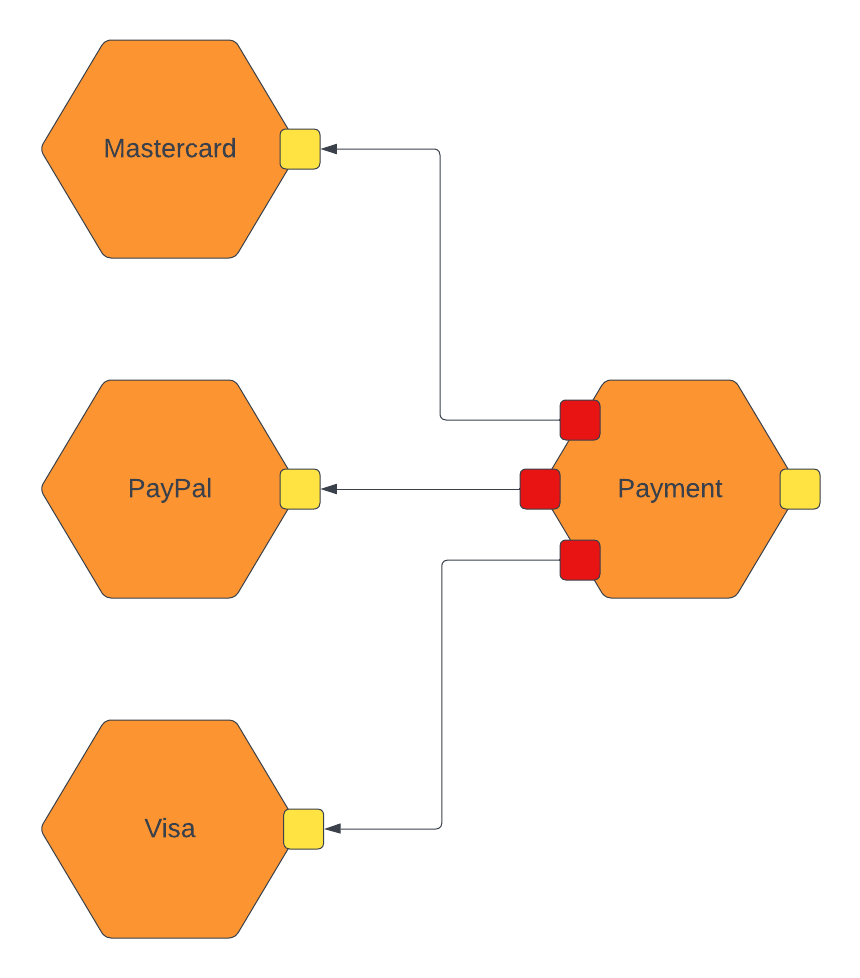
\includegraphics[width=0.5\textwidth]{figures/aggregator_example.png}
    \caption{A group of microservices handling different payment methods. The payment service acts as an aggregator obscuring the underlying services. The orange hexagons depict services, the yellow boxes depict input ports and the red boxes depict output ports.
    Sending a request to the payment service will aggregate the message to the correct payment service depending on the user's chosen payment method. This is done without the client needing to know the correct service's location and protocol.}
    \label{figure:aggregator_example}
\end{figure}
\newdif{Redirection} is a pattern which works similarly to the aggregator, but architecturally is very different.
A service with an input port can specify that a resource name gets redirected to a specific service via an output port.
\cref{lst:redirector-inputport} displays how an input port can specify resources and map them to an output port.
This means that a client sending a request to the redirector can specify a resource name in the communication media, and the redirector will forward the message to the correct service based on that resource name.
To specify a resource name the client simply needs to specify it in the URL, e.g \texttt{socket://localhost:9000/!/rss} where the \texttt{/!/rss} part is what specifies the resource name.

Redirection can be used to implement several different microservice (API) patterns since it essentially is a proxy.
Generally, a lot of API structures can be implemented using redirectors, because of how a client can specify a specific resource.
\text{API Gateway} is one of the API patterns which can be implemented using redirectors, which are used a lot by heavily visited sites like Netflix.\footnote{Optimizing the Netflix API - \url{https://netflixtechblog.com/optimizing-the-netflix-api-5c9ac715cf19}}

\begin{jolisting}[][caption={Input port which redirects requests using resource names}, label=lst:redirector-inputport]
inputPort RedirectorPort {
    Location: "socket://localhost:8888"
    Protocol: sodep
    Redirects:
        rss1 => OP1
        rss2 => OP2
}
\end{jolisting}

A simple example of what the redirector could be used for is: imagine that an e-commerce application wants to have one point-of-entry for the system. The application could set up an \textit{API Gateway} which will act as that point of entry. 
When a client wants to get information for a product page, it can specify what it needs in the resource names. This also handles protocol transformation so the client does not need to know the internal service's required protocols.
The example is showcased in \cref{figure:redirector_example}. The client makes requests to the redirector specifying the resource name to fetch the relevant data.
\begin{figure}[h!]
    \center
    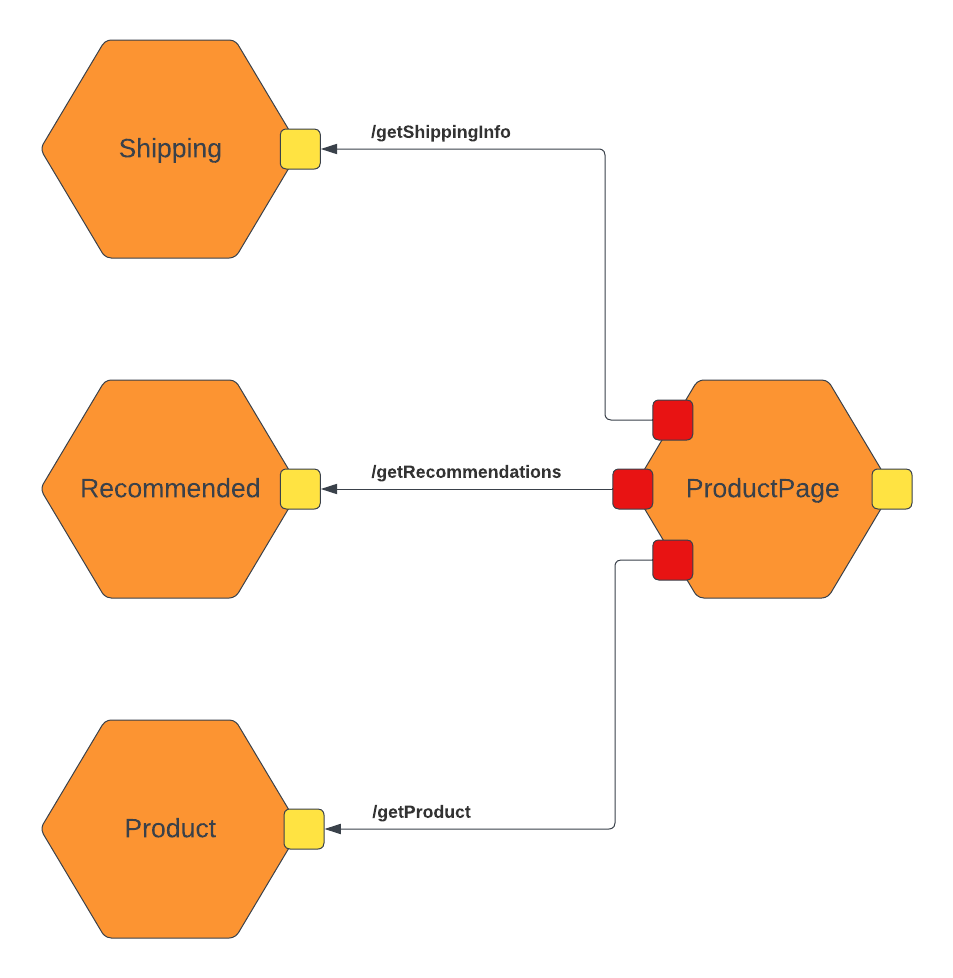
\includegraphics[width=0.5\textwidth]{figures/redirector_example.png}
    \caption{A group of microservices which can be accessed through an API gateway. 
    The client can specify a resource name to specify which service to send the request to.
    The product service fetches information about a product. The recommendation service fetches
    the recommended products based on the user and the shipping service fetches shipping information given the user's location.}
    \label{figure:redirector_example}
\end{figure}
\newdif{Couriers}  allow the developer to append functionality to a set of operations. They work well in extension with other communication topologies like aggregators.
The developer defines a courier process by specifying an input port and a set of operations. When that input port receives a request using any of the operations, the courier process executes some code before forwarding
the request along to the main operation implementation.

Couriers can be used to implement any type of middleware functionality. From the book by Olaf Zimmermann et al., many of the quality patterns can be implemented using couriers. This includes
\textit{conditional requests}, \textit{rate limit}, \textit{pricing plan} etc. Besides the quality microservice API patterns, other microservice patterns can be implemented using couriers, namely, \textit{API key} security and authorization.
\newdif{Collections} is another extension of aggregators. Collections are useful when an aggregator input port aggregates services which share the same interface.
They are specified by grouping output ports when defining aggregates.
This together with courier processes can fully, and easily, implement a load balancer for services sharing interfaces because the courier can forward the requests to any of the aggregated services based on some condition.
Since collections are an extension of aggregates, they can have the same use cases, but the collections can group services that share the same interfaces but can have much different underlying business logic.

\section{Docker \& Docker-Compose}
Docker\footnote{Docker - \url{https://www.docker.com}} is a containerization tool used for deploying applications. It builds an \textit{image} which specifies how the container should build and start when it is created.
Docker handles a single container, and \textit{Docker-Compose}\footnote{Docker-Compose - \url{https://docs.docker.com/compose/}} is used to handle multi-container applications. Docker-Compose will handle the networking between containers, so it is a great tool for testing and deploying applications using a microservice architecture.

Docker-Compose is a container orchestration tool, essentially configuring multiple containers and allowing the developer to ensure that the correct files are mounted, the correct ports are exposed and the containers are bound to their specified networks. It also handles multiple instances/replicas
of containers if needed.

\subsection{Jolie in Docker}
\label{label:jolie_in_docker}
To utilize Docker and Docker Compose when developing a microservice architecture in Jolie, creating images can be done using the Jolie base image \texttt{jolielang/jolie}.
Using this image when making a Dockerfile will set up Jolie when building the image, so only the exposed ports, source files and possible runtime arguments should be handled by the developer.

When running a container, the developer needs to specify what container ports to expose, what parameters should be parsed into the Jolie program, and if it needs to connect to other services the developer needs to first create the network and then assign each container to that network.
This is where Docker Compose, or \textit{Kubernetes}\footnote{Kubernetes - \url{https://kubernetes.io}} which is another container orchestration tool, can become helpful because it will take care of all this if the developer specifies it in the deployment configuration file.

Connecting ports over a Docker network needs some extra work from the developer. Ports which use TCP/IP sockets for communication cannot use "localhost" as seen in the previous examples, they need to use the container name as the host address so Docker can figure out where to send messages inside the network.
This can look something like: \texttt{socket://auth:9999}, where \texttt{auth} is the name of the container.

\section{Current Tools}
Jolie, and other programming languages, do have some tools in order to enhance the developer experience. This section will go through some of the tools
which have been developed for Jolie and then look at some of the counterparts in other languages.
%
\newdif{Joliedoc}\footnote{Joliedoc - \url{https://docs.jolie-lang.org/v1.10.x/language-tools-and-standard-library/documenting-api/index.html}} generates a documentation page for a single Jolie service. This gives an overview of the API a Jolie service exposes. It shows the input ports and output ports of the service as well as their location and protocol.
This tool is useful when the developer wants a simple and easy-to-follow representation of a single service's API, which include operations, types, port information, and dependencies.
For other programming languages, there are tools like \textit{JSDoc}\footnote{JSDoc - \url{https://jsdoc.app}} which look at the comments in the code to generate the API documentation. This requires the developer to write more lines for the same result.
Tools like \textit{Stoplight}\footnote{Stoplight - \url{https://stoplight.io}} and \textit{Swagger}\footnote{Swagger - \url{https://swagger.io}} can do the same for all languages, but this requires the developer to set up a markdown or YAML file and specify the whole API in that.
Because of Jolie's way of writing the API as a part of the language, Joliedoc can infer the API from the code without the developer needing to write more lines or comments to achieve this goal.
Jolie does have another tool which generates OpenAPI specifications, which Swagger uses, but this is more to be used in conjunction with these other tools, and is not a standalone tool like Joliedoc is.
% TODO
\newdif{JPM}\footnote{Jolie Package Manager - \url{https://docs.jolie-lang.org/v1.10.x/language-tools-and-standard-library/basics/package-manager/index.html}} is a package management tool for Jolie which, similarly to NPM, keeps track of dependencies of a Jolie program.

\subsection{Visualization Tools}
There are a lot of different visualization tools for software architecture which all fall into some categories and all have different use cases and intentions.
The subset of tools which fall under the category of \textit{modelling tools} aims to document a system on different levels of abstraction. This can be on the level of individual components to large-scale businesses with interconnecting components and sectors.
Tools like \textit{IcePanel}\footnote{IcePanel - \url{https://icepanel.io/}} and \textit{Aplas}\footnote{Aplas - \url{https://aplas.com/}} allow the developer of a system to use C4 modelling to create a model of their system, on any level of abstraction.

Another subset of tools is the code-based tools which allow the developer to programmatically or textually create models. This is where tools like \textit{mermaid}\footnote{MermaidJS - \url{https://mermaid.js.org/}}, \textit{ELK}\footnote{Eclipse Layout Kernel - \url{https://www.eclipse.org/elk/}} and \textit{graphviz}\footnote{Graphviz - \url{https://graphviz.org/}} belong.
These tools allow the developer to write structured text or code and then they will render the diagram. Developers do not have to use any specific modelling technique, if they can write it in text or code it will be visualized.

The last relevant category of tools is the diagramming tools. Tools like \textit{draw.io}\footnote{Draw.io - \url{https://drawio-app.com/}} and \textit{lucidchart}\footnote{Lucidchart - \url{https://www.lucidchart.com/pages/product}} allows the user to diagram everything from E/R, UML and FlowCharts to complex systems.
This is often done in a drag-and-drop fashion.

One thing all these tools have in common is that they need developers to handle the modelling and diagramming. The developers need to have an overview of the system and then model it using any of these tools.
\clearpage
% Text:              √
% Citations:         √
% Revision:          X
% Final Revision:    X
\chapter{Using the Visualization Tool}
With the foundational knowledge and context for the microservice architecture, microservice patterns, the Jolie programming language, and the current tools both for Jolie and for visualization in general in place, it is time to get familiar with the tool developed for this thesis.

This chapter will go into how the tool is used to enhance the development experience by going through a simple example microservice application.
Firstly, an application is defined. The application for this example is a simple e-commerce platform consisting of seven microservices:

\begin{itemize}
    \item \textbf{User service} - Handles user authentication. Lets the client create, update and delete their account and also log in to get an authentication token.
    \item \textbf{Product service} - Handles product information. This service exposes a basic CRUD (Create Read Update Delete) API for products sold on the platform.
    \item \textbf{Recommended service} - Handles fetching recommended products. A client can query this service which will, based on the user's id, return a list of products which the user might also like.
    \item \textbf{Order service} - Handles grouping of selected products and all the information required for the user to place an order. This includes shipping and tax fees.
    \item \textbf{Payment service} - Handles transactions of orders. When the user places an order they must provide some kind of payment method as well as the necessary information to complete the transaction.
    \item \textbf{Analytics service} - A monitoring service. This service can keep track of popular products, frequent shoppers, what products get bought together, and much more.
    \item \textbf{Notification service} - Handles sending e-mails to users when the transaction is approved. Can also send promo codes, offers, and discounts to users.
\end{itemize}
This example is very simplified, and only the architectural aspect of the microservices will be implemented, meaning the connections between services and the APIs. This means that no business logic will be implemented, and
the types of interface operations will be simplified since the functionality of the application is not in focus in this chapter.
Other details such as deployment, data persistence, and security will also be omitted from this example. A simple diagram can be seen in figure \ref*{figure:full_example_lc} which displays the desired architecture of the application.

To showcase the visualization capabilities of the tool the application will not be developed using any architectural programming features from Jolie such as embeddings, aggregation, redirection, etc.
These will, however, be introduced later.

\begin{figure}[h!]
    \center
    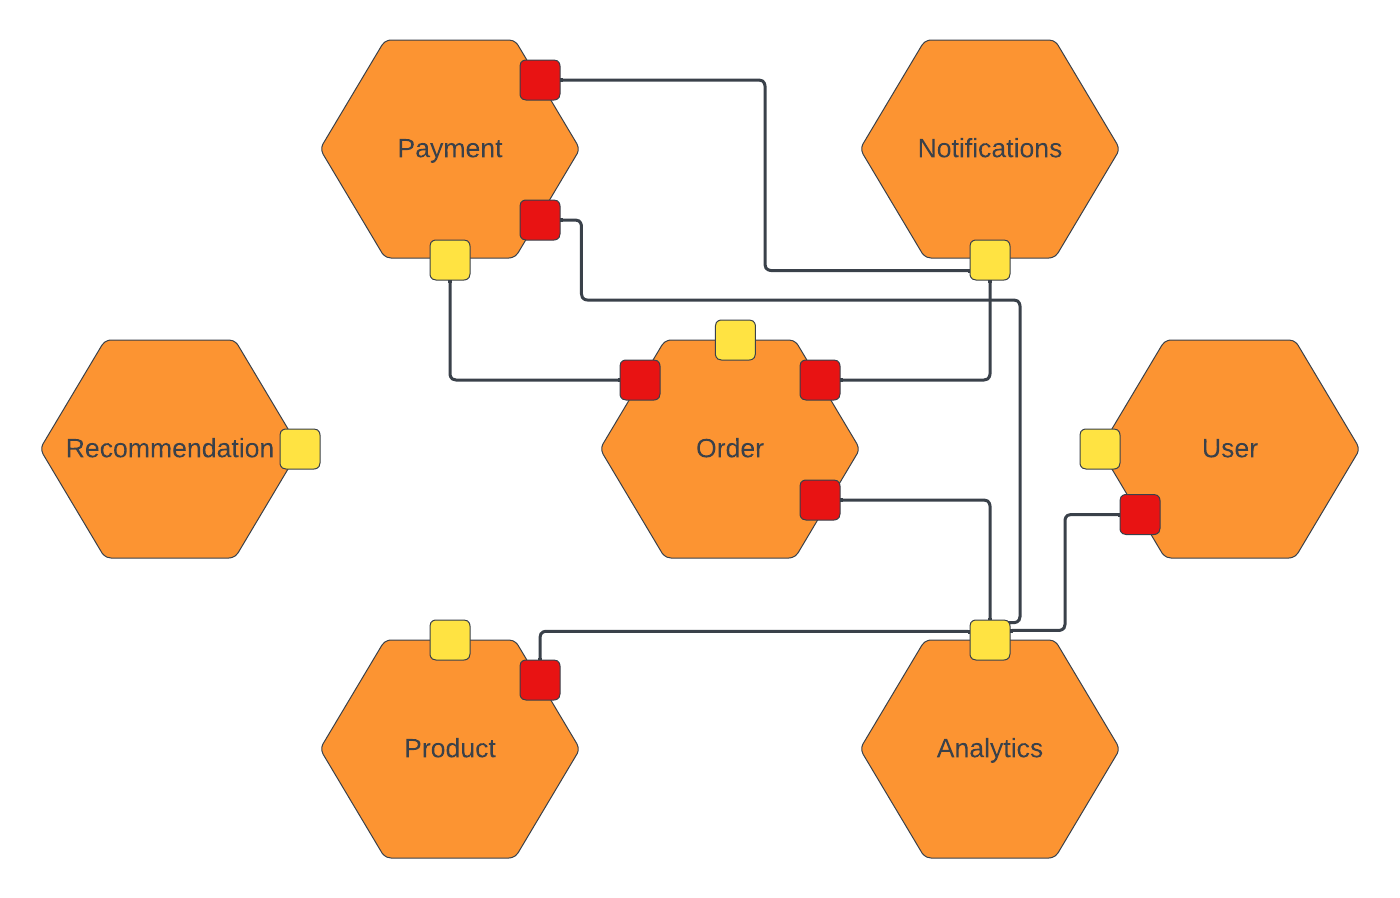
\includegraphics[width=0.70\textwidth]{figures/full_example_lc.png}
    \caption{A diagram of the example architecture of the e-commerce application. The output ports (red) represent internal communication between the services via their input ports (yellow).}
    \label{figure:full_example_lc}
\end{figure}

\section{Setup and Requirements}
In order to use the tool, Jolie must be set up correctly with version \texttt{1.11.0-git}. This section will not specify how this is done, but the Jolie website goes more in detail on how
the correct git version is installed \footnote{Downloading the newest version of Jolie - \url{https://www.jolie-lang.org/downloads.html}}. From this point onwards it is assumed that the environment variables are set correctly to point to the git version of Jolie.

The tool is developed to be used with Visual Studio Code\footnote{Visual Studio Code - Code Editing. Redefined. - \url{https://code.visualstudio.com/}}, aka VS Code, which is a code editor developed by Microsoft.
VS Code has a large ecosystem of plugins which are used to enhance the developing experience.
To start using the tool, it must be downloaded and installed either from the VS Code marketplace under the name: \texttt{\toolname}, or compile the source code and extract a \texttt{.VSIX} file to install manually.

The development starts with creating a \texttt{.JSON} file which \toolname[] uses to know which services are at the top level of the application.
The plugin has a default file name it will look for, namely, \texttt{architecture.jolie.json} located in the root folder, which is where the developer will define all top-level services, networks, and properties of the services.
The plugin comes with a command to initialize the architecture file, and this creates the file and populates it with a template service contained in a network.

\subsection{Structure of the Architecture File}
The architecture file is a JSON file which consists of an array of arrays of services. The outermost array can semantically be understood as the list of all networks.
Listing \ref*{lst:architecture-file-structure} shows this structure where the \texttt{\{...\}} represents the services. Each network can have any number of services, and it is up to the
developer to specify what a network represents depending on where the services will deploy.

\begin{jsonlisting}[][caption={Structure of the architecture JSON file showing two networks.}, label=lst:architecture-file-structure]
[
    [
        { "file": "svc1.ol" }
    ],
    [
        { "file": "svc2.ol" }
    ]
]
\end{jsonlisting}

The services have different properties which the user can specify. All properties are showcased in appendix \ref*{appen:architecture-file-structure}.
For the example in this chapter, only the file needs to be specified for each service, for now.

\section{Developing the Services}
All seven services in this example will have a unique folder each in the root directory of the project. This is done to separate which files are belongs the which service.
In each folder, JPM can be initialized if the developer needs it, and the interfaces, types, and services will all be separated in files as well.

The tool will be utilized as much as possible to create and refactor code, all while every service being developed will be visualized next to the source code in VS Code.
Every time a service has been declared it is added to the architecture file. This can be done quickly by the developer using code snippets added by the tool. All architecture JSON file snippets can be seen in appendix \ref*{appen:vscode_snippets}.
\subsection{The User Service}
The interface which specifies what operations the user service implements is called \texttt{UserIFace} in this example.
Listing \ref*{lst:useriface} shows how the interface is set up. The ErrorResponse type is a more universal response type which gives a message and status code, which can be used in case of an error, but with no error, it will simply set the error flag to false.
Each of the request types represents what data the operation needs, in order to be invoked. For registering users and logging in an email and password are needed. The update request type represents the user to be updated and what is going to be updated for the user. The delete request simply needs the user ID of the user.

\begin{jolisting}[][caption={The interface for the user service}, label={lst:useriface}]
interface UserIFace {
    RequestResponse:
        register(RegisterRequest)(ErrorResponse),
        login(LoginRequest)(LoginResponse),
        updateUser(UpdateRequest)(ErrorResponse),
        deleteUser(DeleteRequest)(ErrorResponse),
}
\end{jolisting}

The service is created in the main file and the execution is set to \textit{concurrent}.
The service can now be added to the architecture file. Since only one service is present in the main OL file, only the file name needs to be specified in the service JSON.
Now the visualization tool can be run using the command \textit{Jolie: Visualize} in VS Code, and a single service called \textit{User} can be seen.

To use the tool to add the ports, double-click on the service to open the service in the sidebar. Next to the empty lists of ports, a \texttt{"+"} button can be clicked to add either an input port or an output port.
This will bring up a pop-up window, shown in figure \ref*{figure:popup_create_inputport}, where the user can specify the details of the port such as name, location, protocol and a list of interfaces.
\begin{figure}[h!]
    \center
    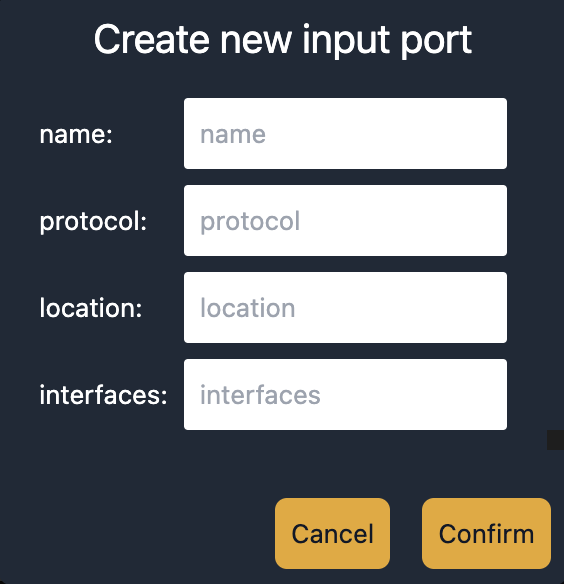
\includegraphics[width=0.35\textwidth]{figures/popup_create_inputport.png}
    \caption{Pop up in the visualization tool where a user can specify details about a port, and by clicking 'confirm' will add that port in code.}
    \label{figure:popup_create_inputport}
\end{figure}

Using this feature. The service needs to have an input port which uses the interface specified before, \texttt{UserIFace}, and before creating the output port for the analytics service, the interface for the analytics service should be defined to prevent a parsing error from the Jolie parser. 
The analytics interface is called \texttt{AnalyticsIFace}, and the operations will be discussed in another section. For now, it is just an empty interface.

After clicking 'confirm' on the popups, the interfaces are correctly imported if they exist. The code for the user service is displayed in
listing \ref*{lst:user-svc}, where some of the implementation details are omitted, but the general structure of the service can be seen.

\begin{jolisting}[][caption={The user service after the ports have been created with omitted implementation details.}, label={lst:user-svc}]
from .userInterface import UserIFace
from ..analytics.analyticsInterface import AnalyticsIFace
service User {

    execution{ concurrent }

    inputPort IP {
        ...
        Interfaces: UserIFace
    }

    outputPort Analytics {
        ...
        Interfaces: AnalyticsIFace
    }

    main {
        ...
    }
}
\end{jolisting}

The implementation details of the types are omitted for all services, but the source code for the application example can be found in the GitHub repository\footnote{Source code: \url{https://github.com/EmilOvcina/jolievisualize/tree/main/microservice_example}}.

\subsection{The Product Service}
The product service handles all operations of the products. This is a basic CRUD service, which also will send analytics to the analytics service, which can be used to monitor popular products etc.
The create and update operation's request types require a product, which is a type containing information about the product, and a user ID because only users who own the product should be able to alter it.
The read operation request type is only an integer corresponding to the product ID. The delete operation request type is a type containing the user ID and product ID to, once again, check if the user is allowed to delete the product and the ID of the product.

When the types and interface (\texttt{ProductIFace}) have been created,
a service named \textit{Product} is created in the main \texttt{.ol} file and once again the execution context is set to \textit{concurrent}.
The service is added to the architecture file in the same network as the user service, and can now be seen in the visualization user interface.

By opening the product service in the sidebar the input and output port can be created similarly to the user service previously. The input port will use the \texttt{ProductIFace} interface and the output port will use the \texttt{AnalyticsIFace} interface.
The two services displayed in the visualization UI can be seen in figure \ref*{figure:jv_product_and_user} with the two ports created for each service.
\begin{figure}[h!]
    \center
    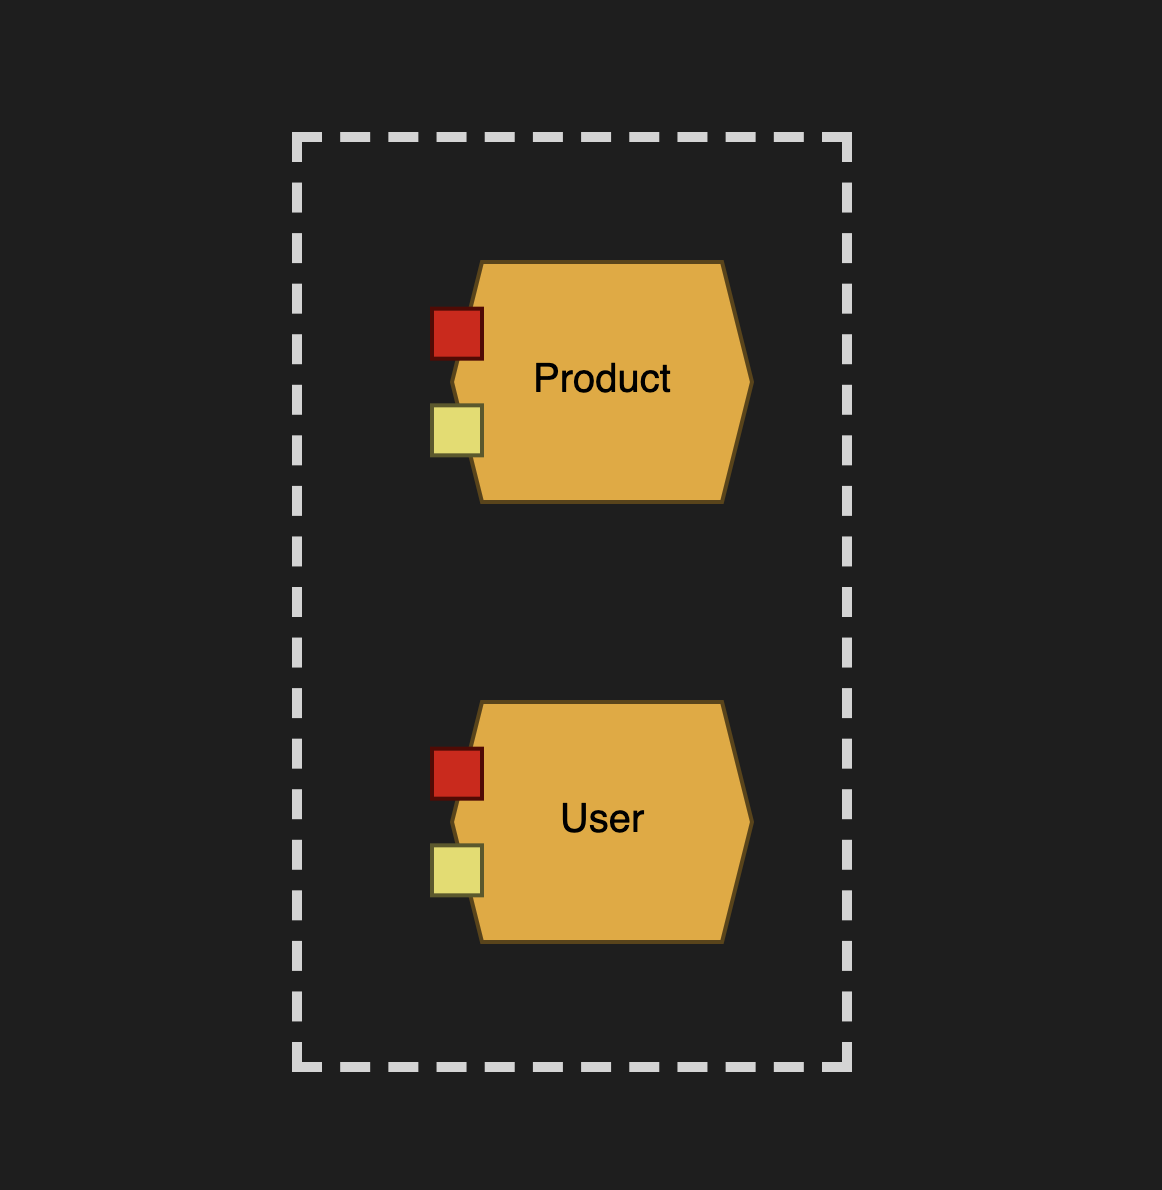
\includegraphics[width=0.5\textwidth]{figures/jv_product_and_user.png}
    \caption{The product and user services displayed in the visualization tool's UI. They have an input port (yellow) and an output port (red) each and they both are considered to be in the same network.}
    \label{figure:jv_product_and_user}
\end{figure}

\subsection{The Analytics Service}
This service supports one operation for now. This is \texttt{addToLogs(AnalyticsRequest)}, which is a one-way operation. The interface for the service is already defined, so the operation is added there with the request type being \texttt{AnalyticsRequest}. This type holds information about what content will be logged and from which service.

This service is created in the main file, and the execution is also \textit{concurrent}. The analytics service is added to the architecture file and is displayed in the visualization UI.
The input port can be created using the tool just like the last two services, and the interface for the
port is \texttt{AnalyticsIFace}.

The input port is using the TCP/IP communication medium, and the output ports in the product and user services must be connected to the input port of the analytics service.
If the ports are not connected in the visualization UI, it is possible to change the location of the ports directly in the UI.
By clicking on the ports, the sidebar will open displaying information about the ports. Double-clicking on the location field allows the user to change it.
Doing this for both output ports to make sure they have the same value in the location field will connect the output ports to the input port in the UI, as well as, change the code to match the changes made in the code.

After connecting the ports, the connections is be represented in the visualization UI. This can be seen in figure \ref*{figure:jv_analytics} where the user and product services are connected to the newly created analytics service.

\begin{figure}[h!]
    \center
    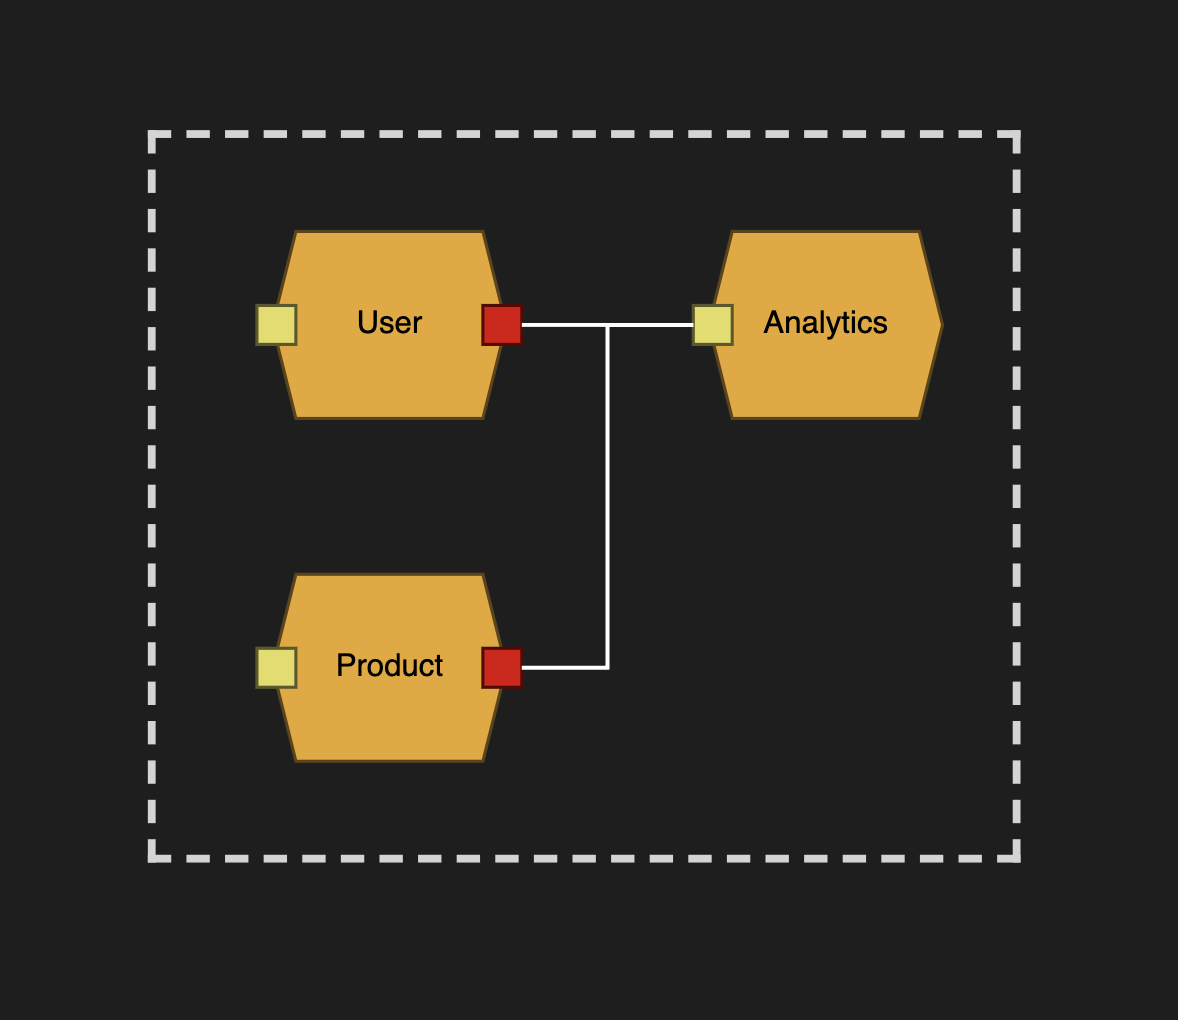
\includegraphics[width=0.5\textwidth]{figures/jv_analytics.png}
    \caption{The product, user, and analytics services displayed in the visualization tool's UI. The user and product services have an output port (red) each of which is connected to the input port (yellow) of the analytics service.}
    \label{figure:jv_analytics}
\end{figure}

\subsection{The Notification Service}
The notification service will get requests from other services and send an email to the specified user. This can be when a transaction is completed, a product is back in stock etc.
This service supports one one-way operation, \texttt{sendNotification}. The request type contains the user ID to send the notification to, and the content of the notification.
Adding the service to the architecture file will render it in the UI.

Using the UI, once again, to add an input port with the interface called \texttt{NotificationIFace}. This is the only port needed for this service.

\subsection{The Payment Service}
The payment service's only job is to process payments from orders. The interface for this service is a single request-response operation, \texttt{processPayment}.
The request type for this operation needs information about the payment method, amount to pay, user ID and credit card details. The response type has an error flag, date of purchase and optionally a receipt if the transaction was successful.

Same with all other services, this is added to the architecture file to render it in the UI. The payment service needs one input port for the interface \texttt{PaymentIFace}, an output port connected to the analytics service, and another output port connected to the notification service.
Once again, by opening the ports in the sidebar, the user can change the location of the ports to match so the correct ports are connected.

\subsection{The Order Service}
This service handles the user's orders. A user can place an order, see that order and cancel it. The interface, \texttt{OrderIFace}, has these three request-response operations: \texttt{placeOrder}, \texttt{getOrder}, and \texttt{cancelOrder}.
The request type of placing an order requires a list of products and a payment request, which could be populated by the shopping basket in the application UI.
The response type simply lets the user know if the order was placed correctly with an error flag and a status code. The "get order" operation requires an order ID of the order to return and will simply respond with an order type containing information about the order.
Cancelling an order also requires the order ID and will respond with a type with an error flag and status code.

When the order service is defined in the main file, and the service is added to the architecture file, the input port is created using the \texttt{OrderIFace} interface.
The service needs three output ports. One for the analytics service, one for the notification service and one for the payment service. The analytics that the service can log is what products get bought together and how many orders a user cancels etc.
The notification service needs to be invoked to send confirmation about cancelled orders, or if the status of the order changes.
The payment service will be invoked through the order service, so when the user places an order the payment service will get the request and send the response back to the order service which creates a response for the client.

The tool can either help in connecting the correct ports as done with the other services, but the developer can do that in the code as well, and when the developer does a change in the code manually and saves the document, the visualization UI is automatically updated to reflect the changes made in the code.

\subsection{The Recommended Service}
The last service is a standalone service, which only the client needs to invoke.
The recommended service interface consists of one request-response, \texttt{getRecommendations},
which based on the user ID given finds the most recommended products as a list of products.

A possible extension to the service can involve fetching analytics data from the analytics service and doing calculations with that information to avoid sharing databases between services. This will require the analytics service to expose an operation allowing the internal services to get the data, and an output port in the recommended service to invoke that operation.
This extension will be omitted in this example.

\subsection{The Completed Application}
With all services and ports in place, the application can be seen as one microservice architecture in the visualization UI, as seen in figure \ref*{figure:full_example_lc}.

Having the whole application in the visualization tool allows the developer to inspect the application in detail to get an overview of what is happening between services and what APIs the different services expose.
Clicking on ports opens the sidebar and displays information about the ports including the interfaces. All the interfaces can be clicked on to further inspect the operations in the interface. All types used for the operations are also clickable and will display information about the type,
including the subtypes, cardinality and root type.

From here the developer can start using architectural patterns in Jolie as discussed in the previous chapter. Some refinements of the current services can also be made, for example, the payment service should probably have underlying services to take care of different payment methods.

\begin{figure}[h!]
    \center
    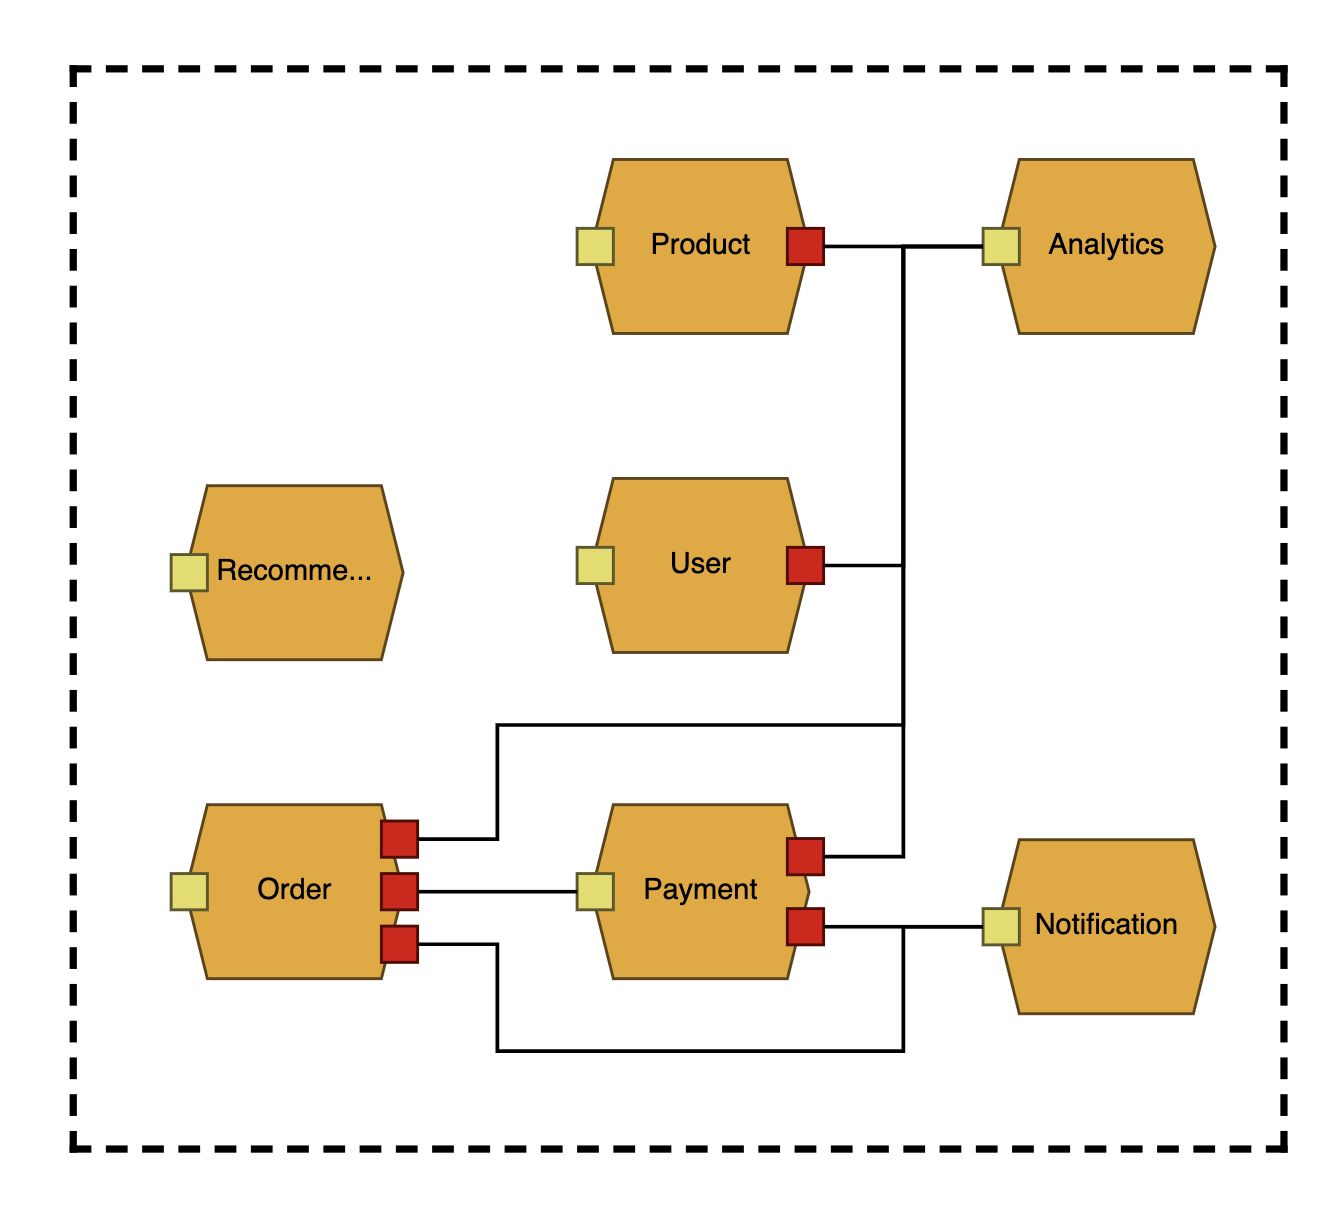
\includegraphics[width=0.8\textwidth]{figures/jv_completed.png}
    \caption{The entire e-commerce application is displayed in the visualization tool's UI. All services exist in the same network and all are top-level.}
    \label{figure:jv_completed}
\end{figure}

\section{Improvements}
Now that the application has all seven services implemented, the developer can apply some of the architectural features allowed in Jolie to improve the application and implement some of the microservices (API) patterns discussed in the last chapter.

\subsection{Embedding}
It is not necessarily the best idea to have all seven services as top-level services. The services not accessed by the client directly should be embedded in the services which need them.
The analytics service is used by four services: Order, Payment, User, and Product. To embed the analytics service in these four services the input port's location can be changed to \texttt{local}. This is just one way of embedding using local in-memory communication and is not the only way of embedding services. Another method of embedding will be used for another service later.
Changing the port location to \texttt{local} can be done in the sidebar.
The output ports in the mentioned services using the analytics interface must also be deleted which, at the moment only can be done in the code, but instead of looking for the main files which contain the ports,
opening the port in the sidebar and clicking \texttt{\{\}} at the top of the sidebar opens the correct file in the editor.

Now in the architecture file, for the analytics service, the field \texttt{instances:4} can be added to the JSON object representing the analytics service. This will add 4 instances of the analytics service, and by using the mouse and dragging the services, the developer can 
drag the services onto the four services and embed them one after one. This will add the code in the correct files to specify that the analytics service instances are embedded.

The notification service is also used by other services, and should not be accessed by a client directly. For this service, the ports will not use local in-memory communication as the analytics service did.
In the architecture file the notification service will need to have two instances, so the field for instances is added to the service JSON. Now two instances of the notification service exist as top-level services. Each instance can be dragged into its respective
parent service, namely, the order and payment services and the embedding code will be added to both services. The embedding will use the already existing ports to connect so no local ports will be created.

The last service to embed is the payment service in the order service. This can be done by either changing the existing port to use local communication or just dragging the payment service
as it is now into the order service to use the existing ports as communication and the code will again be changed to reflect the embedding.

The new architecture can be seen in figure \ref*{figure:jv_embedded} and it shows only the services which are accessed by a client. The services which now have embeddings can be seen with a little "plus" sign, which can be clicked on to expand the visualization of the service revealing local ports and embedded services.
The embedded services can be removed by dragging them out of their embedder. Doing this with local communication will cause the local ports to be removed from the code.

\begin{figure}[h!]
    \center
    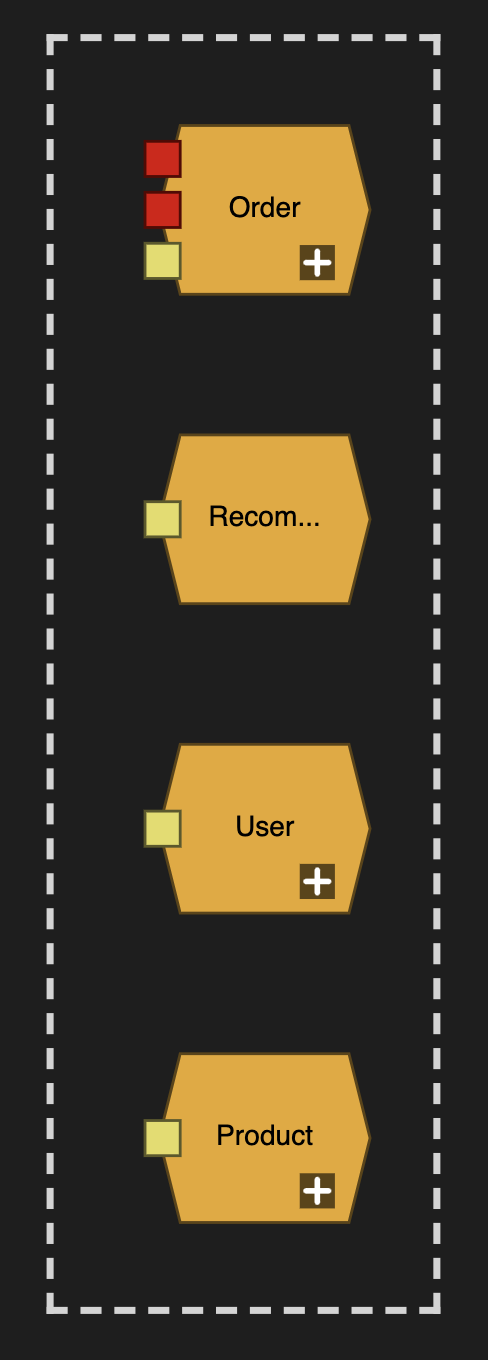
\includegraphics[width=0.17\textwidth]{figures/jv_embedded.png}
    \caption{The e-commerce application after the payment, notification, and analytics services have been embedded.}
    \label{figure:jv_embedded}
\end{figure}

\subsection{Aggregation}
Now all the top-level services are services which a client is directly requesting. It is now possible to add some of the architectural patterns to the system in order to implement some of the ideas mentioned in the previous chapter.
The tool facilitates the possibility to select services by holding the shift key and clicking the service shapes. The sidebar will show which services are selected and a list of patterns which can be applied based on some
criteria. Selecting the four top-level services of the example application shows that the aggregator pattern is applicable.

Clicking on the "aggregator" button will open a pop-up allowing the developer to enter all necessary information for creating an aggregator service, and choosing if the aggregator should connect to existing ports or create new input ports for the aggregated services, or if the aggregated services should be embedded in the aggregator service.
For this example, the aggregator will just connect using the existing ports requiring that the developer types in the locations of the input port for each service correctly.
After clicking "confirm", the aggregator service will be created in the file of the first service selected. The new architecture can be seen in figure \ref*{figure:full_example_lc} and shows that the aggregator service called \texttt{Aggregator} is connected to the services and is displayed in a slightly more orange colour 
to illustrate that the aggregator is a generated service and is only a scaffolding service which the developer needs to implement the functionality for.

\begin{figure}[h!]
    \center
    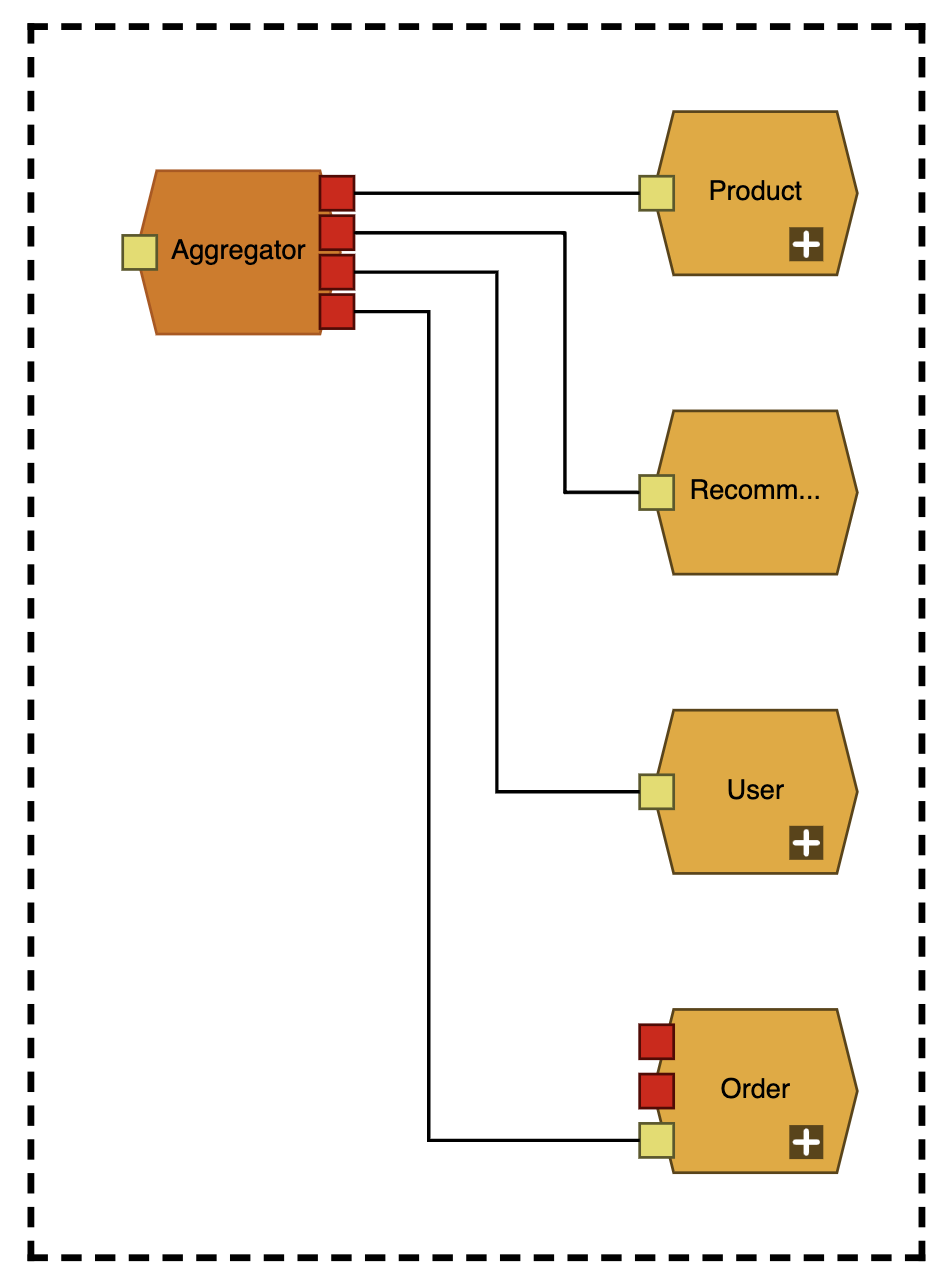
\includegraphics[width=0.41\textwidth]{figures/jv_aggregator.png}
    \caption{The e-commerce application with an aggregator service that serves as a reverse proxy for the services that are invoked by clients.}
    \label{figure:jv_aggregate}
\end{figure}

\subsection{Networks}
The final part of the application is determining which networks each top-level service belongs to. This is relevant when the application is deployed.
The services can be dragged out of their dashed box to create a new network and place the service in the network.
Other services can then be dragged into the new network to add the service to that network, or services can be dragged out of their network to create more networks.

Creating new networks and moving services around to different networks does nothing in the Jolie code. It changes the structure of the architecture file, but that is only for visualization purposes. 
For this example, the networks can be arbitrary so the services will all reside in the same network for now.

\section{Prototyping}
The tool facilitates testing in a local deployment. Using the command \textit{Jolie: Docker-Compose} will generate a build folder where all top-level services reside in their respective subfolder containing all dependencies, a package.json file if the project is using JPM, and a Dockerfile to create an image when running the deployment.
A \texttt{docker-compose.yml} file will also be generated specifying each service and the deployment configurations.
In the generated deployment file the networks are also specified and added to each service depending on what network the developer added the service to in the architecture file and what networks the service is connected to via ports.
This is just a generic deployment file and should not be used for anything other than testing the application locally.
The tool only supports Docker-Compose at the moment, so Docker is required for this feature to be effective.

To make the Jolie service accessible from outside clients it is required that the services follow the requirements for running Jolie services in Docker mentioned in the preliminaries section about Jolie in Docker \ref*{label:jolie_in_docker}.
This includes changing the location to use the container name as the hostname if TCP/IP communication is used between services and adding an extra field in the architecture file.
The field is a \texttt{ports} field which is a list of Docker ports the container will expose using the syntax of Docker ports, e.g. \texttt{"3000:3000"} meaning that port 3000 is exposed externally and mapped internally to port 3000.
Other fields can be added to customize the deployment. The container name can be changed using the field \texttt{"container"} giving more freedom in terms of what the services are called in the code
because the default container name is the service name. If a service in the deployment needs any dependencies outside of Jolie, e.g. configuration files, a list of files can be specified in a \texttt{"volumes"} field.
This will add the files to a resource subfolder in the build folder and will be bind mounted when the container is running.

In the architecture file, external dependencies can also be added to the architecture which allows other services to be displayed alongside the Jolie services. The developer can specify a service in a network and give an \texttt{image} field
which links to an image on Dockerhub or other image repositories. In the visualization UI, this will be shown with a blue shape which indicates that it is an external service, and the ports also need to be specified in the architecture file.
Building the Docker-Compose file, external services are also added.

When everything is set up and docker is running on the machine, the developer can start the local deployment with Docker-Compose by running \texttt{docker-compose up} in a command line tool or terminal.

% Text:              X
% Citations:         X
% Revision:          X
% Final Revision:    X
\chapter{Implementation}
The tool has now been used in a practical example to give an idea of how it is used to enhance the development experience.
This chapter will go into the design decisions and implementation details to make each part and feature of the tool function, as well as,
explain what the tool consists of and how the components work together to create the finished product.

The specifics of the code will be omitted, but the general control flow of each part of the tool will be explained.

\section{Overview of the Components}
The tool essentially consists of four components: The VS Code extension, the user interface written in Svelte, the \javatoolname[] program and a wrapper program for \javatoolname[] which uses NodeJS called \nodetoolname[].
The \javatoolname[] program is used to run the Jolie parser, which is also written in Java, and that will gather all information from the Jolie code needed by the visualization tool.

The Svelte user interface is the component which takes in the user input and renders the services, ports and connections.
In order for the UI to get the relevant data from the Jolie code, the VS Code extension invokes the \nodetoolname[] program, with the correct parameters, which invokes the \javatoolname[] program.
\nodetoolname[] program listens for the output of the \javatoolname[] program,

meaning that the \nodetoolname[] program functions as a wrapper for the \javatoolname[] program so the VS Code extension does not have to invoke \javatoolname[] directly,
and sends the data to the VS Code extension, which sends the data to the user interface.

Figure \ref*{figure:init_tool_sequence} shows the process of initializing the tool in VS Code, which is done using the \textit{visualize} command in VS Code.

\begin{figure}[h!]
    \center
    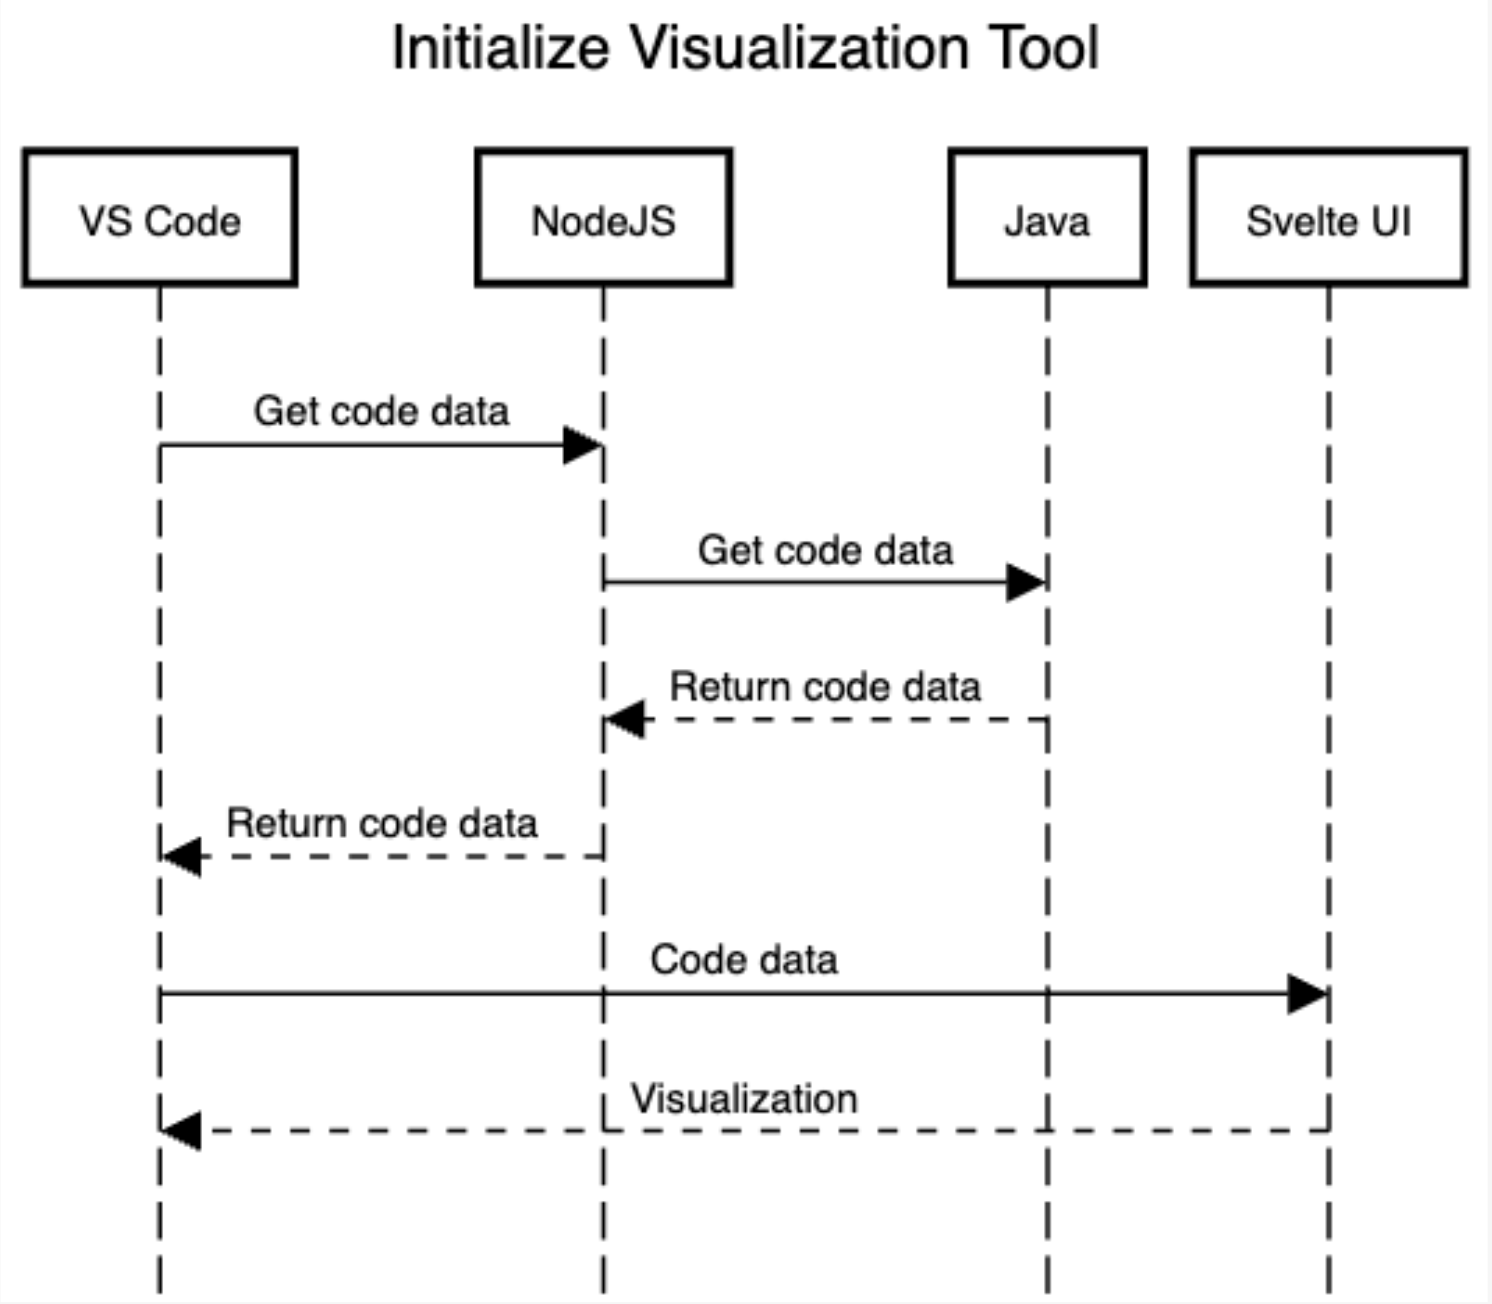
\includegraphics[width=0.70\textwidth]{figures/init_tool_sequence.png}
    \caption{A sequence diagram showing the sequence of requests and invocations between the four components that the tool consists of. The VS Code extension invokes the \nodetoolname[] program using NodeJS which will handle running the \javatoolname[] program with the correct parameters, and afterwards, the VS Code extension sends that data to the UI which will visualize it in VS Code.}
    \label{figure:init_tool_sequence}
\end{figure}

\section{Data Representation}
The data which the \javatoolname[] program will output is consistent through all
four components of the tool. The chosen data format is JSON data because it is easy to parse in TypeScript, which all components consist of.
The data needed for the tool is a list of interfaces, a list of types and the list of services.

\subsection{Interfaces \& Types}
Each interface in the list of interfaces has a name, identifier, file path, and two lists of operations.
One of the lists contains all one-way operations, and the other contains all request-response operations.
The request-response operations consist of the operation name, the request type name-file path pair and the response type name-file path pair, and for one-way operations it is similar but with the response type omitted.
Having the type name and file path pair and a separate type object list instead of the type object directly in the specific interface object is a design decision made at the very start of the development process.
Each interface could have a list of types which will save computation when the user clicks on the type in the sidebar and the type is displayed because only the interface's list of types needs to be searched for the correct type.
This, however, has the drawback of a lot of duplication, only if all interfaces in the system use a unique set of types can this issue be avoided.
This is why a global list of types is used. The interfaces then reference what types are used for operation and the global list of types can be used when using the sidebar to view interfaces and types, and by
using the Jolie language constraint of no duplicate type names in the same OL file, the file path and type name are enough to find the correct type when searching for it.

The list of types, as mentioned, contains all types used by all interfaces in the architecture.
Each type object in the list represents the information about a type in the code, this includes the name of the type, the file in which the type is defined, the root type, subtypes which is a list of types as well, and cardinality of the type in case of this being defined.
If the type is a \textit{choice type}, the two choices are also represented in the type object as strings which reference other types in the global list.\footnote{Types in Jolie - \url{https://docs.jolie-lang.org/v1.10.x/language-tools-and-standard-library/basics/data-types/index.html}}
Types from \textit{interface extenders} are also added to this list.

An example of the JSON data used to represent interfaces and types from Jolie can be seen in appendix \ref*{appen:joliejson_iface_types}.

\subsection{Services \& Networks}
The last list in the global JSON is the list of services. The list of services is also used to infer how the networks are set up and which services reside in each network.
This approach draws inspiration from how bigraphs are used to model software architecture. Bigraphs are a type of graph consisting of two sub-graph components. The link graph and the place graph. The link graph models the connection between nodes in the system while the place graph models the topology.
The nodes in the system of the bigraph can be directly mapped to Jolie services. Bigraphs also model ports which are a component of Jolie services as well.
The data representation used for the tool draws the most inspiration from the place graph since the link graph is inferred by the locations and protocols of the ports in Jolie.
A place graph models the topology and the networks, which are called \textit{roots} in bigraph terminology, and also embeddings, which are called \textit{nestings}.
The bigraph inspiration is taken from \textit{The Space and Motion of Communicating Agents} by Robin Milner \cite{BigraphBook}, where bigraphs are formally introduced and explained but are not necessary for this use-case.

The place graph component can be seen as a list of trees where the root is the network and contains all top-level services as immediate children and embeddings of the top-level services are the children of those services.
This fits well with how a Jolie system can be modelled, so the list of services in the global JSON is essentially a place graph or a list of trees where each node is a service in the system.
Each root in the list of trees is a network. In the sense of JSON, the network is a list of services since it can have any number of children, and the \textit{embeddings} list of each service is also a list of services.

The services in the JSON also need to contain all other information which is used by the tool.
This includes the input and output ports, execution target, name, identifier, and file path but also the information specified in the architecture file, which is container name, volumes, parameters etc.

An example of the JSON data used to represent services and ports from Jolie can be seen in appendix \ref*{appen:joliejson_services}.

\subsection{Architectural Programming}
The architectural programming features in Jolie also need to be represented in the data to visualize it in the tool's UI.
This includes couriers, collections, aggregations, and redirections. All of these aspects are created at the Jolie port level in the code, so the information is also represented in the ports of the JSON.

Aggregations in the JSON are represented by the name of the output port to aggregate to, optionally the aggregate can have an interface extender and which be defined here.
Collections are essentially a list of aggregations, so collections are also represented in the aggregates as a list of names of the output ports, and because multiple output ports of one service cannot have identical names, this will not create ambiguity.

Couriers are defined in Jolie based on an input port with aggregation, so the port also represents the couriers of that port.
The couriers in the JSON have lists of operation names and interface names which the courier will act upon. This is both for request-response and one-way operations. The names refer to the operations and interfaces in the system.

Redirections for an input port are a list of pairs of resource and output port names. This represents how a resource is redirected to an output port.
However, since the resource of the redirect is defined using the location of the output port, the output port will not be connected correctly unless the resource part of the string is removed, so the resource part of the location, namely,
the part after \texttt{/!/} is removed and placed in a separate field in the JSON for the output ports.

All types of architectural programming features in the JSON representation of Jolie can be seen in appendix \ref*{appen:joliejson_architecture}.

\subsection{Prototype Data}
The data used to create the prototype is also represented in JSON and is split into two parts, the Docker-Compose YAML file content and the service folders which contains the Jolie files, dependencies, and Dockerfile.
The Docker-Compose file content is simply a string, which will be written to the file. The build folders are used to generate this string, but this will be explained more in detail in a later section.
The services folders, which are called build folders internally, are an array of objects that each represent a folder to be created when generating the prototype.
The build folders have to represent what a Docker image will contain, so each folder can be seen as a Docker image. This has to be independent of the Jolie code since two identical services can have different parameters or runtime arguments.

Each build folder contains a list of files which will be added to the folder itself, but also a list of files which will be added to the shared resource folder.
Information such as runtime arguments, exposed Docker ports, and the service name is also added to the build folder JSON because the Dockerfile needs this information when it is being generated.

The JSON data generated to create the prototype can be seen in appendix \ref*{appen:joliejson_prototype}, but with omitted docker-compose YAML content.

\section{The \nodetoolname[] Program}
% why it is created and how it works
The \nodetoolname[] program functions as a wrapper for the \javatoolname[] program. It is created so the VS Code application does not have to execute the \javatoolname[] program directly and also if the tool should be extended to other code editors or run in the browser, this functionality should not be implemented in the VS Code extension.
The \nodetoolname[] program also makes sure to return errors if a parsing error occurs or if Jolie is not installed correctly.

This part of the tool consists of three parts, the data fetching part which executes the \javatoolname[] program and checks for errors, the server part which allows the developer to visualize their program's architecture directly in the browser but without the code refactoring functionality, and
prototyping which is identical to the functionality in the VS Code extension, but this can be used if the user of the tool installs only this part of the tool without the VS Code extension.
The server uses the express framework\footnote{Express Framework - \url{https://expressjs.com/}} to open an endpoint to get the JSON data and also serve the webpage as static assets on localhost.

\section{The \javatoolname[] Program}
% how the data is fetched in the Java tool
The \javatoolname[] program is written in Java and is used to gather the required information from the Jolie code. The Jolie parser is written in Java and therefore the \javatoolname[] program here uses the parser directly to get the abstract syntax tree nodes and create the JSON objects.

The \javatoolname[] program has two types of outputs which is used by the tool. The JSON representation of the entire system and the information used by the prototyping functionality. Both functionalities of the \javatoolname[] program require the whole system to be parsed using the Jolie parser.
Firstly, the tool creates the networks by parsing the architecture JSON file and making an internal representation of what it contains. The networks contain a map of top-level services mapped to a \texttt{ServiceNode} which is the abstract syntax tree (AST) node of a service from the Jolie parser. The top-level service is a representation of a Jolie service in the architecture file, as seen in appendix \ref*{appen:architecture-file-structure}.
The \javatoolname[] program uses a lightweight JSON library, \textit{json-simple}, to parse files and create JSON objects\footnote{JSON-simple - \url{https://code.google.com/archive/p/json-simple/}}.
To get the ServiceNode AST node from the parser, the Jolie parser is invoked using its module parsing method. This returns the whole AST of a file, called a \textit{program}. All ServiceNodes are then captured and added to the network's map object.

When the networks have been created, depending on if the program should send visualization data or prototyping data, all the necessary information about the services, ports, etc. is created.
\subsection{Parsing the Jolie System}
A system inspector has been created in order to parse the networks.
The system inspector uses the created list of networks containing the top-level services and ServiceNodes.
The inspector goes through each network's map object and creates a service object which is an internal representation of the services used by the tool.
It creates the services by looking at all the child nodes of the ServiceNode AST node in a loop and using type comparison to check what child node is being looked at and how to parse the information correctly.
Relevant child nodes for a service are: \textit{ExecutionInfo}, \textit{CourierDefinitionNodes}, \textit{EmbedServiceNodes}, \textit{InputPortInfo}, and \textit{OutputPortInfo} nodes.

Service objects can also have a list of services which are considered embeddings. When looping through the AST nodes of a service, embedded service nodes will be used to create services, which are added to the parent's list of services instead of the global list of services.
This will enforce the place graph structure of services mentioned in the data representation section.

The most complex of the child nodes are the two types of port nodes. Input and output ports also have an internal representation in the \javatoolname[] program which keeps track of all the necessary information about the ports used by the tool.
Ports have to contain information about the location, protocol, name, interfaces and operations.
When the ports are being created, the interfaces which are used by the ports will also be created. These interfaces are also represented internally and will store information about the operations.
The operations are also parsed using type comparison, since two types of operation declaration AST nodes exist in Jolie, namely, request-response and one-way.
The interfaces are added to a global object \textit{JolieSystem} which has information about all parsed services and interfaces.

For input ports specifically, information about aggregates, couriers and redirects is also stored. Redirects can be seen as a mapping where a resource is mapped to a port name. This is how the Jolie parser represents redirects as well, so this is simply copied over to the tool's representation.
Aggregates are simply a name of an output port but can contain collections and interface extenders, however, Jolie's internal representation of aggregates contains this information so the interface extender just has to be created to match the tool's representation of interfaces, and collections are a list of output ports which will be copied directly.

When the interfaces are created the types used in the operations are also parsed and created in an internal representation.
This representation stores information about the root type, cardinality, subtypes, etc.
The types in Jolie can also be three different AST node types, namely definition links, inline definitions and choice definitions. Type comparison is also used here to parse the type correctly depending on the AST node type.
Types are, similarly to interfaces, added to the system's global list of types.

Each building block of a Jolie service has an internal representation in the \javatoolname[] program and all of them have a \texttt{toJSON} method which takes all information stored in the objects and creates a JSON object.
When the tool invokes the \javatoolname[] program to get the JSON data, the \texttt{getJSON} method is invoked on the global JolieSystem object which cascades and invokes the getJSON method for all internal objects which also carcades to its internal objects.
This will result in a JSON object which resembles the data representation discussed in the previous section, and this JSON can be used by the other components of the tool.

\subsection{Generating the Prototype Data}
The \javatoolname[] also creates data for making the prototype. This includes the content of the Docker-Compose YAML file and the information needed for creating the service folders and the resource folder.
After the whole system has been parsed and a JolieSystem is created, the system will be given as a parameter to a \textit{build} object which will handle the logic for creating the JSON data.
The builder will first create the service folders using the services in the networks from the JolieSystem object. Duplicate build folders will be checked for at this stage, which is done to make sure that duplicate images will not be generated when using Docker-Compose.
However, as mentioned in a previous section, two identical services can be two different images if the runtime arguments are different, which is also handled here.

After the build folders have been created as internal objects, they are parsed onto another object which builds the Docker-Compose YAML string. The JolieSystem is also used here to create the networks in the Docker-Compose file.
The Docker-Compose builder also has some internal representation of what a service is, since two services in Docker-Compose can use the same image but have different deployment properties, which means that they should be created as separate services in Docker-Compose, but they will not have two different service folders.
The Docker-Compose builder uses a string builder to create the YAML file content. It goes through all services and creates an internal \textit{compose service} and like with the service folders, composes duplicates and counts replicas.

The networks are also created in the Docker-Compose YAML, which can have another semantic meaning from the networks defined in the architecture file.
In Docker-Compose networks are used to restrict services connecting, which is not a problem with a system created in Jolie, so to have the Docker-Compose networks work similarly to how networks in the tool work, each service in Docker-Compose is set to be a part of
its network, as specified in the architecture file, but also all other networks that the service has a port connecting to.\footnote{Networks in Docker-Compose - \url{https://docs.docker.com/compose/networking/}}

\section{Visualization User Interface}
After the JSON data has been created using the \javatoolname[], it needs to be rendered in a user interface, which can handle user input as well.
There are two aspects of these components, firstly, how to create a reactive user interface which can handle user input and handle updates based on how the user interacts with the tool. Secondly, how the components of the architecture are rendered efficiently and how they should be laid out to make the architecture readable and manageable.

\subsection{User Interface}
The tool's user interface is essentially a static webpage where the JSON data is loaded when the site is initialized.
The UI uses CSS for styling and JavaScript for the logic, like most standard websites.

However, creating a very feature-heavy reactive user interface in standard CSS and JavaScript is almost impossible in a reasonable amount of time.
The first improvement to the development of the UI was to replace JavaScript with TypeScript (TS).
TS is a compiled and strongly typed programming language, created by Microsoft, which is a superset of JavaScript. It compiles directly to JavaScript which makes it usable by the UI webpage.
Some of the benefits of using TS include type checking, self-documenting code, interfaces, and generally enhanced productivity.\footnote{TypeScript - \url{https://www.typescriptlang.org/}}

Writing standard CSS can also be a very tedious process, so to enhance the development experience TailwindCSS, or just Tailwind, is used.
Tailwind is a CSS framework which aims to move CSS to the HTML components. CSS properties are defined in the class attributes of the HTML components where readable class names have been defined meaning that any combination of these classes can be used to style components.
Tailwind also defines a design system which a developer can use to enforce a standard when it comes to the design of the UI, and with tools like \textit{postcss} and \textit{autoprefixer} the build size of the utility CSS components will be kept at a minimum.\footnote{TailwindCSS - \url{https://tailwindcss.com/}}

\subsection{Rendering \& Layout}
All services, ports and edges between ports are rendered using SVG components.
Different SVG\footnote{SVG Elements - \url{https://developer.mozilla.org/en-US/docs/Web/SVG}} elements are used for different parts of the UI. Polygons are used to render service shapes, rectangles are used to render ports and paths are used to render edges between ports.
SVG elements in HTML are easy to manipulate in TS, so when the JSON data is loaded in, the correct HTML components are created and then TS is used to create the SVG data for each component so they get the desired shape and size.
To help with the manipulation of SVG elements in TS, a library is used called \textit{D3.js}.\footnote{D3.JS - \url{https://d3js.org/}} D3 has a long list of features to help visualize data using SVGs, however, the only functionality used for this tool is
the ability to select SVG components and apply attributes, event handlers, and stylings.

The problem with D3 is that it has no way of doing the layout of the services and ports.
To ensure that the architecture is always readable from the UI, and the connections of ports are visualized practically, a framework/library is used.
The framework needs to support the visualization of embeddings, networks and connections between ports.

Different frameworks were tested to see which gave the best results while providing the capabilities needed for the tool.
The first framework tested was MermaidJS\footnote{MermaidJS diagramming tool - \url{https://mermaid.js.org}} which is a diagramming and charting tool. Mermaid uses markdown to represent components in a diagram and does the rendering and layout of the components. Using this tool would mean that D3 was no longer necessary, however, MermaidJS uses D3 internally for the rendering along with Dagre-D3\footnote{Dagre-D3 - \url{https://github.com/dagrejs/dagre-d3}} for layout.
The problem with MermaidJS is that it is not generic enough, it supports rendering and layout for a long list of specific diagram types, but none of the types would fit the rendering of services in a microservice architecture.
MermaidJS can draw simple graphs which could work as a foundation for the tool, but this is wasteful. The framework has a lot of capabilities which would go unused.

As mentioned, MermaidJS uses Dagre-D3 for the layout of components, which is the next framework tried for the tool.
Dagre is a graph layout library which primarily focuses on the layout of directed graphs. Dagre-D3 provides rendering using D3 on top of the base Dagre library.
Dagre and Dagre-D3 are both deprecated libraries, even though it is still used by many including MermaidJS.
The problem with Dagre-D3 is that the scope of the library is directed graphs, and nothing more.
Embeddings are not possible to represent.
It is possible to have \textit{Clusters}\footnote{Dagre-D3 clusters - \url{https://dagrejs.github.io/project/dagre-d3/latest/demo/clusters.html}}
but the clusters work more like a grouping of vertices in a graph and not like a vertex having vertices inside it, which is essentially how the embeddings should be represented if a graph library is to be used.

Another library that was also tried but has many of the same drawbacks as Dagre-D3 and MermaidJS is Cytoscape.\footnote{CytoscapeJS - \url{https://js.cytoscape.org}}
This library is also a graph visualization and layout library. It comes with a lot of features out of the box like animations and dragging of the vertices. The main issue of this library is that embeddings are
not possible, but also that many of the built-in features do not fit the visualization tool.

The framework that was chosen for the tool is Eclipse Layout Kernel (ELK)\footnote{Eclipse Layout Kernel - \url{https://www.eclipse.org/elk/}}
which is a layout framework with a collection of different layout algorithms. ELK supports embeddings, ports and edges. This is essentially everything the tool needs for the layout capabilities.
ELK only does layout, however, so a rendering needs to be done by a separate library, where D3 was chosen to render the components of the architecture when ELK has done the layout.
Figure \ref*{figure:elk_example} shows a system being laid out using ELK.

\begin{figure}[h!]
    \center
    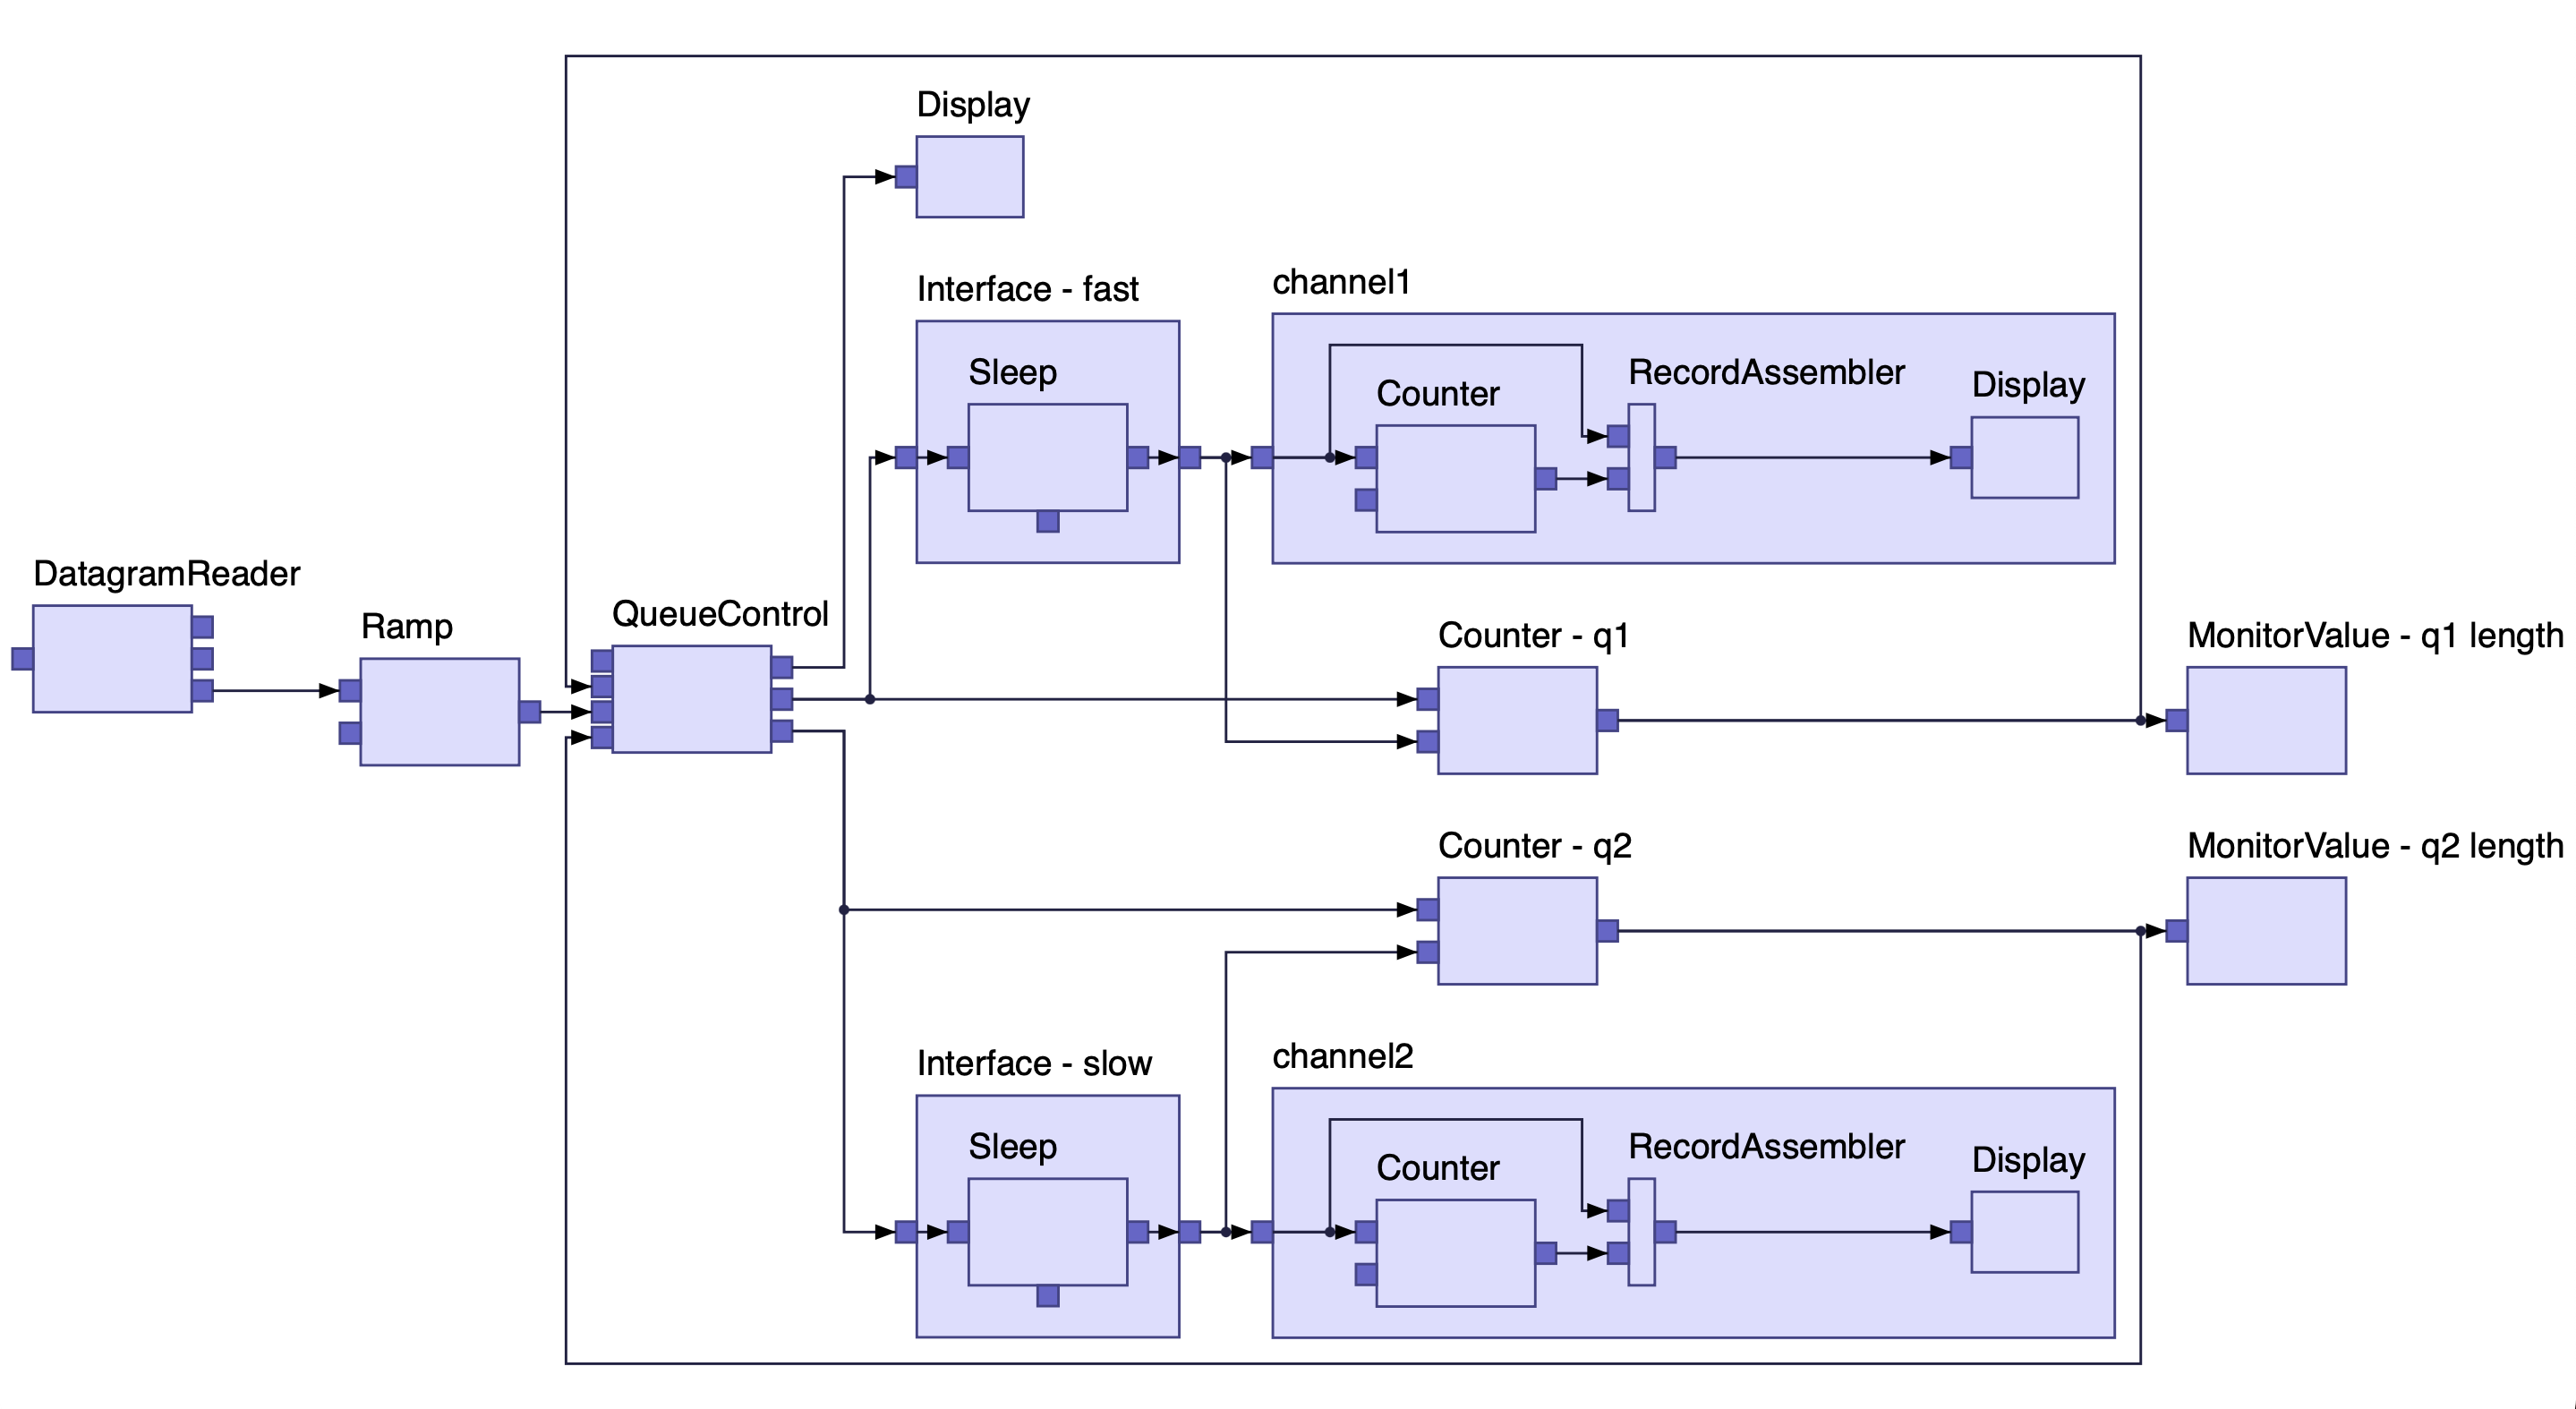
\includegraphics[width=0.80\textwidth]{figures/elk.png}
    \caption{A system using ELK to layout each component of the system including ports and embeddings. Connections between ports are also calculated. The rendering of the system is not done using ELK. Source: \url{https://www.eclipse.org/elk/img/example_layout_complexRouter.svg}}
    \label{figure:elk_example}
\end{figure}

The drawback of using ELK is that in a highly reactive UI, the user might want to position the services themselves, which is not yet possible with ELK.
So when the components of the architecture have been positioned in a network, for example, a service cannot be positioned inside the network. It can however be moved outside the network to move it to another network.
The drawbacks of using ELK do not outweigh the benefits. Having direct support for ports and embeddings is very valuable for the tool, and that is why it has been chosen as the layout framework.

ELK has a TypeScript version, so it can easily be used with the rest of the user interface. To make ELK calculate the layout of the JSON data from \javatoolname[] it needs to be converted into a format which ELK understands.
ELK has a textual graph DSL but also supports a specific JSON format, which is used by the tool because of simpler conversion.

\begin{jsonlisting}[][caption={The ELK JSON format}, label={lst:elk_json}]
{
    "id": "root",
    "layoutOptions": { "algorithm": "layered" },
    "children": [
        { "id": "n1", "width": 30, "height": 30 },
        { "id": "n2", "width": 30, "height": 30 },
        {
            "id": "n3",
            "width": 30,
            "height": 30,
            "ports": [
                { "id": "p1", "width": 5, "height": 5 },
                { "id": "p1", "width": 5, "height": 5 }
            ]
        }
    ],
    "edges": [
        { "id": "e1", "sources": [ "n1" ], "targets": [ "n2" ] },
        { "id": "e2", "sources": [ "n1" ], "targets": [ "n3" ] } 
    ]
}
\end{jsonlisting}

When the UI receives the JSON data containing the networks with services, the ELK graph is created based on the JSON data.
The networks are the children of the root node of the ELK graph. This is specified in the \texttt{"children"} field of the ELK JSON.
ELK nodes in the graph have a field for ports, which are positioned around the node when the layout algorithm is invoked.

To connect the ports with edges, edge objects can be added to the ELK nodes. Embedded connections will be placed in the parent's edge list in the ELK graph, and inter-service connections will have edges in the network containing the services.
Multiple local output ports are handled so the UI can differentiate between local output ports when embedding and disembedding services to avoid removing unwanted ports or rendering connections between ports which should not be there.
This is done in a preprocessing step when the UI gets the Jolie system JSON, where local input ports will be matched to the corresponding output port of the embedder and the location will be unique between the two ports to remove ambiguity.
Connections that are happening between networks are placed at the root of the ELK graph. To determine what edges should be added to the graph, all output ports will be checked to see if a matching input port exists anywhere.

When the ELK graph has been populated with the necessary nodes and edges, the layout is calculated. All the components of the graph get a position and size, and all edges get a list of points. D3 can then render the graph components.
The ELK JSON represents what is rendered in the UI, so embeddings of the top-level services are not added to the ELK graph. When the user of the tool expands a service the embedded services will be added to the ELK graph and
everything gets recalculated and then they are re-rendered correctly in the UI. Generally, every time the user does something in the UI which requires the ELK graph to be modified, the layout algorithm is run.

\subsection{UI Framework}
To facilitate the reactivity needed for the UI when the user starts manipulating the architecture, a UI framework called \textit{Svelte}\footnote{Svelte - \url{https://svelte.dev/}} is used.
Svelte is a framework used to create reactive web interfaces similar to React, Angular, and Vue. The benefit of using Svelte instead of any of the other frameworks mentioned is that Svelte compiles into highly efficient JavaScript,
whereas most of the other frameworks ship some sort of DOM manipulation engine alongside the code. Svelte is the chosen framework because it must run in VS Code which runs in Electron\footnote{Electronjs - \url{https://www.electronjs.org/}}, and the speed is a factor in this case.

Svelte is component-based and works by combining stylings, markup and JavaScript/TypeScript into one file type. Svelte allows the injection of JS variables into the markup, and updating the variables will force a redrawing of the DOM, which makes the user interface reactive.
The user interface is composed of a component tree where the "app" component is the root which holds information about the current ELK graph. Figure \ref*{figure:component_tree} shows the component tree of the user interface. The sidebar and popup window are child components of the root app component, meaning when they are updated, the DOM is re-rendered. 
The parent component also contains the SVG parent component which holds all shapes of the system.
The ELK graph is used here to create network child components. The network components take in the corresponding subgraph as input, which the network can use to create the service and edge child components.
The service components also have edge components which represent the internal edges which connect output ports to the input ports of embedded services.
The zoom component which handles the scaling and transposition of the SVG is also added to the root component to enhance user experience.

\begin{figure}[h!]
    \center
    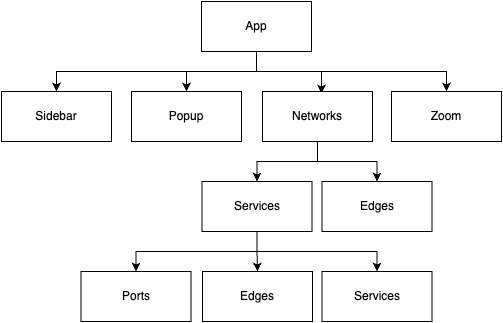
\includegraphics[width=0.70\textwidth]{figures/component_tree.png}
    \caption{The component tree of the user interface created in Svelte. When the root component is updated an update is cascaded down the component tree.}
    \label{figure:component_tree}
\end{figure}

All components in Svelte have lifecycles which are utilized to render the components with D3.js.
The lifecycle loop consists of four stages where all of which have event handlers directly accessible in the TypeScript code in Svelte files. This means that each component can run code at any stage of its lifecycle.
The four events are: \textit{before update}, \textit{on mount}, \textit{after update}, and \textit{on destroy}.
\textit{Before update} happens before anything else. It runs every time the component is updated and before the DOM is created.
\textit{On mount} runs only once when the component is created and runs right after the DOM is created. 
\textit{After update} runs after the DOM is created and runs every time the component is updated.
Lastly, \textit{On Destroy} runs once when the component is destroyed.\footnote{Svelte lifecycle functions - \url{https://svelte.dev/docs\#run-time-svelte}}
All components of the graph will have position and size when they are created because ELK has done the layout at that point.
So when creating the DOM elements for each component, the size and position are already known.
Components which are rendered with D3 have an "after update" event handler which will run \textit{after} the DOM for the component is created. This code will use D3 to render the desired shapes.

The \textit{before update} event handler is used to map the ELK graph component to an object from the Jolie system JSON, because it runs before the DOM is created, it can be used to check if a service component is expanded or not, which allows the DOM of the service to change.

The whole component tree does not re-render if a service is changed by the user. Only when the ELK graph in the root component is updated, will the whole component tree be re-rendered. To make sure that the ELK graph is updated when a service or port is changed, an event dispatcher is used to 
send events up the component tree. Ports and services can send events which their parents listen for and will aggregate towards the root. When the root gets a specific event, it will trigger the ELK layout algorithm and re-render the whole component tree.

The last Svelte-specific concept used is \textit{stores}.\footnote{Svelte stores - \url{https://svelte.dev/docs\#run-time-svelte-store}} Stores in Svelte are global states which can be used by all components of the program. Stores can be written to, which overwrites the object saved in the store, and they can be subscribed to by components which will run some code every time a store is changed.
In this UI, stores are used to keep a state of what is displayed in the sidebar and popup window. This allows all components of the application to write to the store and determine what is displayed in the sidebar or the popup window. 

\section{Visual Studio Code Extension}
The VS Code extension generally consists of the activation events, contribution points and a web view.
The activation events determine what will activate the extension. An example could be that would be when a certain file type is opened, the plugin is activated.
For this extension, the activation events happen by commands which the user can type into VS Code. The commands are displayed in appendix \ref*{appen:vscode_commands}.

The contribution points\footnote{Contribution Points in VS Code - \url{https://code.visualstudio.com/api/references/contribution-points}} are declarations of enhancement that the extension does. There is a long list of different functionalities which can be extended.
This extension's contribution points only include snippets. The snippets are used when creating the architecture file. The snippets work by suggesting auto-completion in JSON files, where the user can press the tab key to jump to different points in the inserted code to quickly edit.
The list of snippets from this plugin can be seen in appendix \ref*{appen:vscode_snippets}.

The last overall part is the web view that VS Code facilitates.\footnote{Webviews - \url{https://code.visualstudio.com/api/extension-guides/webview\#scripts-and-message-passing}} The web view can be used to fully render web content in the editor.
This can be seen as an iframe within VS Code. When the web view is created custom HTML can be set. This HTML can reference JavaScript and CSS code from the host machine's local resources, meaning that the compiled JavaScript and CSS from the user interface made in Svelte, can be used directly in the VS Code extension web view.
This is done by having the extension install the JolieVisualize node package and referencing the compiled code in the \texttt{node\_modules} folder.

The extension can send messages to the web view using a post message function which sends serializable JSON data to the web view.
The JavaScript running in the web view can create an event listener which listens for messages. The payload of the messages declares what type of message is sent and then the web view can act accordingly.
This is useful when the UI should update based on some event in the editor.

% todo something about initializing the extension - flow diagram - wait until name of node program exists

\subsection{The VS Code API \& Commands}
VS Code exposes an API\footnote{VS Code API - \url{https://code.visualstudio.com/api/references/vscode-api}} with a long list of operations and events
which is used in this extension to handle all inputs from the UI, and the code editor.
The API is split into different namespaces where this extension primarily uses the \texttt{workspace}
namespace. This includes all operations and events regarding folders and files in the working directory.
Specific events and operations will be explained more in detail when discussing their applications in this extension.

The built-in commands\footnote{VS Code Commands - \url{https://code.visualstudio.com/api/references/commands}} which VS Code provides can be programmatically executed.
Many of the commands use \textit{providers} to define how they are implemented. This means that the commands essentially execute a provider which can be implemented by the language server protocol (LSP).\footnote{Language Server Protocol - \url{https://microsoft.github.io/language-server-protocol/}}
Providers can also be implemented in the extension or any other extension.
This is useful because the extension can invoke LSP functions programmatically. How the LSP can be utilized for this tool will be discussed in a later section.

\subsection{Live Updates}
When the user of the tool changes something in the code while the tool is running, the visualization reflects the changes done in the code.
Two event listeners are used to keep the UI up-to-date with the code when a change happens in the code. \texttt{OnWillSave} and \texttt{OnSave}.
\texttt{OnWillSave} is an event which fires when the user saves a document but before the \texttt{OnSave} event is fired. The purpose of this event listener is
to check if a service name of a service which is declared in the architecture file has been changed. If the name of a service was changed, the event listener updates the architecture file content to reflect the change before moving on to the \texttt{OnSave} event listener.

The \texttt{OnSave} event listener is used to check if the architecture is updated in the code, if the code was updated in the UI, the listener will not be executed. The event listener also checks the architecture file to see if that has any changes.
If the architecture file has been changed the event listener simply invokes \nodetoolname[] and gets the new JSON data and sends it to the UI to be rendered.
If a Jolie file has been changed the \nodetoolname[] is invoked and the JSON data is checked to see if it matches the data currently used by the UI. If not, the new data is sent to the UI to be rendered.

\subsection{Code Refactoring}
To facilitate the refactoring of code from the UI, the JSON data also needs to contain information about where certain components are in the Jolie source code files.
This is done using the \textit{parsing context} from the Jolie parser. When the Jolie parser creates the AST it keeps track of where tokens are in the file and what ranges a code block spans over.
This information is saved in the JSON which \javatoolname[] creates as ranges with a name indicating what the range spans over.
Listing \ref*{lst:code_ranges} shows how the code range is saved in the Jolie system JSON.

\begin{jsonlisting}[][caption={JSON representing a code range created by the Jolie parser}, label={lst:code_ranges}]
{
    "ranges": [
        {
            "name": "svc_name"
            "start": {
                "line": 21,
                "char": 10
            },
            "end": {
                "line": 22,
                "char": -1
            }
        }
    ]
}
\end{jsonlisting}

All refactorable components in the code must have a corresponding code range. Protocols,
locations and port ranges for input and output ports must be saved in ranges, as well as, embedding code and service names.

When the user makes an edit in the UI, this can be either creation of ports or the renaming of properties, the UI sends a message to VS Code using the VS Code message API, with the necessary data for the refactor. This includes
the code range, the new text and what file it happens in. VS Code has an API to create \textit{workspace edits} which will add or replace text in code using internal position and range representations.
VS Code has an internal object which represents a code range, which is used by the VS Code API to make workspace edits. This is not identical to the code range representation created by the Jolie parser.
This means that conversion needs to happen when the code range is used in the VS Code extension.

When the edit has been created internally it is not yet applied to the document, because it is often the case that multiple edits should happen when a change happens in the UI.
All edits are saved to a list, and when the last edit request comes from the UI, the whole list of edits is sorted according to position in the file, so the edits which are applied further down the document gets applied first to keep the positions and ranges intact for the other edits not yet applied.
After the edits have been applied, the reflected changes can be seen in the source code as well as the UI.

This functionality is used for all types of edits done in the UI, including embedding and applying architectural patterns, to make all edits atomic without having to make specific interfaces for all types of edits possible. 
This allows reusability of the refactor requests, and also the possibility to send multiple refactor requests without suffering from outdated code ranges and latency.

Another type of edit can be used when renaming symbols, like service names, interface names, type names, or port names. This must be done carefully because these names can be imported by other files which means that the names must be updated everywhere.
The LSP specification provides functionality for renaming a symbol which must be implemented by the language server protocol implementation for Jolie.
VS Code can execute this function using the built-in command highlighted earlier. This needs a position of the symbol and what the new name is. The LSP then returns a list of workspace edits which can be applied directly in VS Code.

\subsection{Embedding \& Disembedding}
The user of the tool can drag around the services in the UI, and by dropping them on top of another service or outside the parent service, it will embed or disembed respectively.
Much like the code refactoring functionality, when the user changes the architecture of the system, the UI sends a group of requests which contains the necessary information to reflect the change in the code base.

% Todo something about what happens on the UI side, and how that is reflected in VS Code
% Todo - also the different cases and how they are handled.

% Todo auto import of services, interfaces and types here

\subsection{The Aggregator Pattern}
Applying architectural patterns, like the aggregator pattern, is more extensive than the other operations discussed so far.
Potentially a lot of ports need to be created, as well as, a whole service which needs to be added to the architecture file.

% Todo something about what request is sent from the UI, and how VS Code handles it.
% Todo - mention the case with existing ports, local ports (automatic embedding) and base case.

\section{Prototyping}
% generating docker-compose files
% getting dependencies
\subsection{Dependencies}
\clearpage
\input{chapters/synthesis.tex}
\chapter{Discussions \& Conclusions}
The implementation details of the tool have been explained in depth. Some of the design decisions which has been made during the development of the tool have also been briefly discussed.
This discussion chapter will go into the details of the development process, and elaborate more on what else was tried and tested to achieve the current result.

This chapter will elaborate on the important discussion topics being made throughout the development process of the tool, and explain how
some of the bigger design decisions were made.

The chapter will also discuss what similar tools exist and how this tool compares to them. Lastly, how the tool can be developed further to enhance user experience, and what features and changes could be made to either make the tool more useable
or solve more problems for the user. This will also serve as a discussion of the shortcomings of the tool.

All sections of this chapter will also have a small conclusive part to each of the aspects. This means that no separate conclusion chapter will follow this chapter. However, this chapter will end with a short conclusion of the thesis.
\section{Reconnaissance}
The tool has been through one major revision before reaching the state it is in now. This section
will explain the \emph{first version} of the tool, briefly how it was implemented, and why the revision was needed.
The first version served as a way to get familiar with visualization and D3.js. It was also a tool where different approaches were tested to see what works and what does not.

The general structure of the tool was very different. The first version tried to be more decoupled from VS Code than what the tool currently is.
The first version was a Java program which had an open server socket. From this server socket, a lot of endpoints were exposed which would serve the whole user interface as well as provide the Jolie system JSON data.
This approach requires that a port is open on the machine whenever the tool is running.

It was never tested with VS Code so it is not certain how VS Code would incorporate a tool like this. One idea is
that the tool must be running on the host machine, essentially as a server, and a client in VS Code would need to fetch the user interface from the specific endpoints.
The client in the VS Code extension would be a web view as it is at the moment.
Whenever an update to the Jolie code is made the client in the VS Code web view will have to fetch data from all endpoints again.

\subsection{The Program Inspector}
To get the JSON data from the Java service, an internal \texttt{ProgramInspector} was used to fetch the information about the Jolie services. This inspector exists within the Jolie parser but has limitations with how it gathers information about services.
It looks at a file and gathers all information meaning that if multiple services exist in one file, the ProgramInspector will not differentiate between components in one service and components in another service.
When the ProgramInspector has gathered all the AST nodes of a Jolie source file, the JSON objects are created directly. No internal representation of each component was created for this version of the tool.

Another problem with the first version is that no sense of top-level services is present. The tool simply parses all files in the root directory recursively. This creates a lot of bloating of the visualization and JSON data because unwanted services, interfaces, and types may be present in the user interface.
This resulted in all services, both top-level and embeddings being in one global list of services.
This is ultimately why the architecture file is introduced. So the user can specify exactly what services in what files should be parsed and visualized in the user interface. The other benefit of the architecture file is that the user of the tool can specify parameters for the visualization and prototyping of the services.

\subsection{User Interface}
In the first version of the tool, the user interface is vastly different. A lot of inspiration was taken from the documentation of Jolie.\footnote{An example of how services are displayed in the Jolie documentation - \url{https://docs.jolie-lang.org/v1.10.x/language-tools-and-standard-library/architectural-patterns/synchronous-vs-asynchronous/index.html}}
This shape of services is easy to implement because they all have a direction, all input ports are on one side and all output ports are on the opposite side.

\cref{figure:old_ui} shows a very early version of how the user interface displayed the service shapes. This is without any layout algorithm being applied to the service which is why all services are next to each other.
The red triangles on the left side of the service shapes represent the output ports and the yellow squares on the right side represent the input ports, and the height of the service is simply determined by how many ports it needs to fit.

The problem with this approach is that in some architectures, the visualization can be very hard to understand.
It gives the sense that there exists some sort of direction or flow between services which is not necessarily the case.
Embeddings are not represented intuitively. If a service is embedded by another service it is simply placed to the left of the embedder service and a dashed square is drawn around the two services indicating that an embedding is happening, but it 
is not clear to an inexperienced Jolie developer what is the embedder service and what is the embedded service.
This is why the current version of the tool has chosen a more \emph{traditional} approach to the service shapes. It does not imply a flow and it can be easier to visualize more complicated architectures.

The UI for the first version is grid-based where all services can be moved around and will snap to the grid.
The reason a grid is used is that the edges that represent the connection between ports are calculated using the \emph{A*} pathfinding algorithm,\footnote{A* pathfinding algorithm - \url{https://en.wikipedia.org/wiki/A*_search_algorithm}} so each point in the grid is essentially used as a point in a graph that the pathfinding algorithm can use.
This also means that invisible walls are created around the services and ports to ensure that paths do not go through other services or ports.
The current version of the tool has hexagons as service shapes, so to facilitate the possibility of having ports on all sides of the shape, the pathfinding from the output port to the input port must be handled differently.
One idea which was tried is connecting services instead of ports, and then drawing the port shapes at the edge of the service shape where the connection intersects the service shape.
A grid is not used in the current version of the tool because ELK is used to make the edges between ports.

\begin{figure}[t]
\center
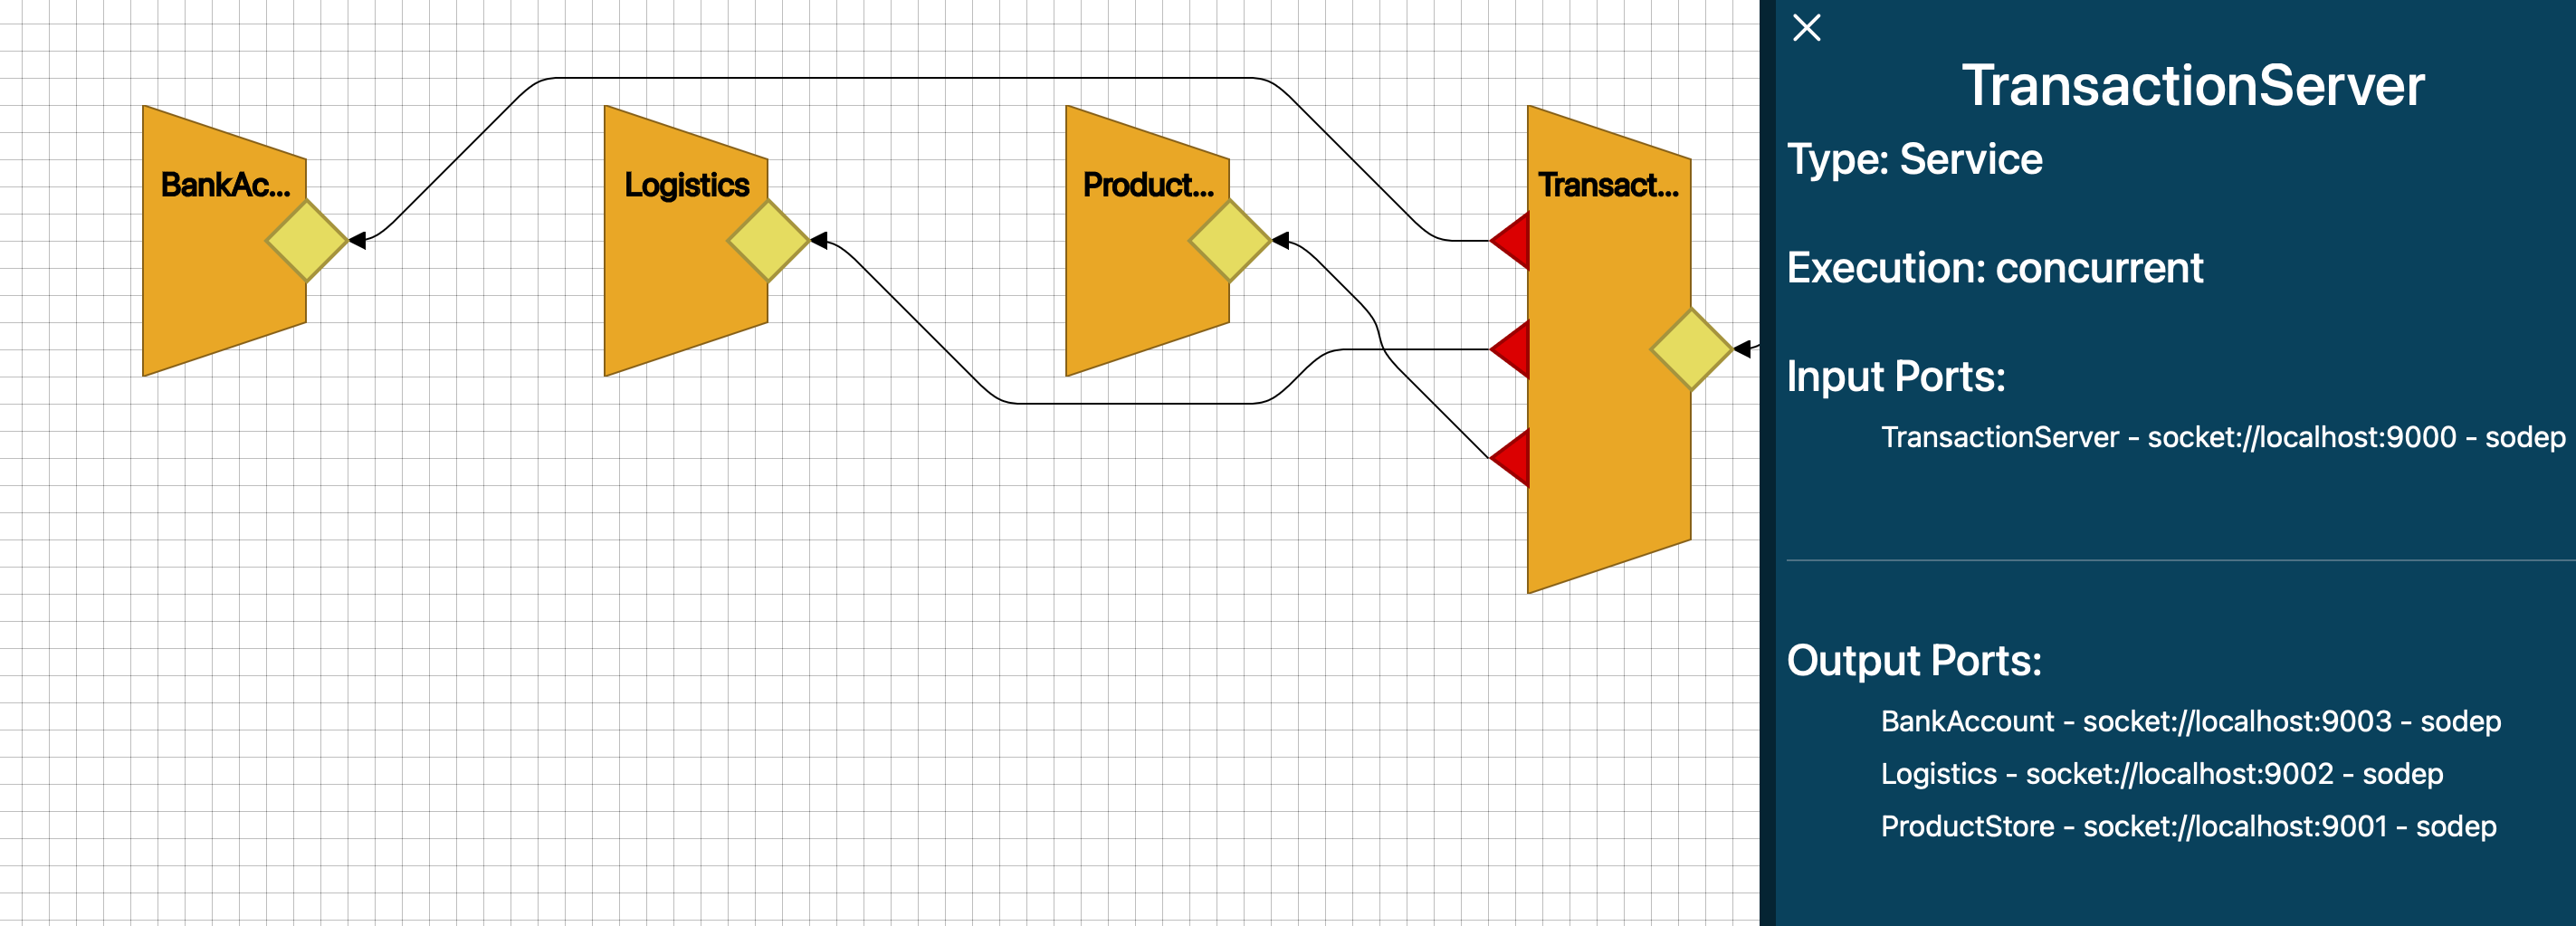
\includegraphics[width=0.8\textwidth]{figures/old_ui.png}
\caption{A very early version of how the first version of the tool displayed service shapes (orange) and the sidebar (blue). No layout algorithm is used to place the services correctly on the grid in this version.}
\label{figure:old_ui}
\end{figure}

\subsection{Layout Algorithm}
The first version of the tool uses a simple custom layered layout algorithm. This is possible because the services have a direction.
The algorithm works by placing each service in a horizontal layer based on how many of each port it has. The starting number of layers is determined by the width of the screen and each layer has a set height limit so when services exceed the limit an adjacent layer is created.
Services with only one input port are placed in the left-most layer, and services with only one output layer are placed in the right-most layer.
The services in between will be ordered so the service with the most connected ports will be placed in the middle-most layer and services with an input port connected to an output port of the middle service will be placed to the left. Services having output ports connected to input ports of the middle service are placed to the right.

This algorithm is very simple. It worked on the handful of tested examples from the Jolie GitHub repository.\footnote{Jolie Examples on GitHub - \url{https://github.com/jolie/examples/tree/master}}
But when the system becomes more complex connection-wise, it can quickly break or incomprehensible. One advantage of using this algorithm is that the user can drag around the services if the initial layout is bad.

The algorithm does not necessarily break because of the hexagon shapes which were introduced after. The switch to ELK was made because connections can become complex, and having a highly customizable framework is much safer in terms of the systems the tool will potentially have to visualize.
ELK uses a variety of researched layout algorithms which are more robust than the simpler layout algorithm which was used before.

\subsection{UI Framework}
The introduction of a UI framework was made because of the component tree, lifecycle events, and reactivity. Before Svelte was used to create the user interface, it was created in pure TypeScript.
The UI in the first version has no lifecycle events. All JavaScript code is loaded after the DOM is created.
The flow of the user interface is that after the DOM has loaded all the Jolie system JSON data is loaded and preprocessed very similarly to the current version, but here, the custom layout algorithm is used.
Then all components are added to the DOM, under one parent container, using \emph{jQuery}\footnote{jQuery - \url{https://jquery.com}} and rendered using D3.js. Lastly, the event listeners are added to the system components. The event listeners include the mouse listener for moving the service shapes around and opening the sidebar to display information about the components.
When the user interface is updated by the user, a re-rendering happens. Since all system DOM elements are added under one parent container element, that specific element is simply cleared and the rendering is invoked to populate it with the updated elements.

This approach of using pure TypeScript/JavaScript is not inherently wrong. After all, Svelte compiles down to optimized JavaScript.
There are general benefits and consequences of using a UI framework. Some of the important benefits are efficiency in handling reactivity, reusable components, and enhanced maintainability.
Efficient reactivity means no manual manipulation of the DOM is necessary. The code will update the state of the components which automatically updates the DOM.
Some of the consequences of using a UI framework are the learning curve, performance, and framework-specific limitations.
Some UI frameworks have a steep learning curve, especially for newer web developers, so having to learn and understand the framework can in some cases take more time than just implementing the functionality in JavaScript.
The performance is not necessarily a problem for Svelte since the overhead is minimal, but for larger UI frameworks like React and Angular, performance can become an issue since they ship a virtual DOM\footnote{React virtual DOM - \url{https://legacy.reactjs.org/docs/faq-internals.html}} which in VS Code can be a bottleneck.
For this specific tool, there are no apparent framework-specific limitations with Svelte, which is one of the reasons it was chosen.

\section{Control Flow}
Having a simple control flow between the components of the tool is key to preventing bugs, keeping the tool fast, and making the tool easier to extend and maintain.
Different flows were tested to see which gave the best results in terms of speed but also the experience from the perspective of the user.
The first version did not have many flows. The initialization was simple but this version of the tool did not have refactoring capabilities, so comparing it with the current solution is unnecessary.

The current flow has split up the different operations so they happen both in the user interface and the code simultaneously, without interfering with each other. Another approach which was tried is to have the user interface update from the newly refactored code. This means that when the UI sends a refactoring request to VS Code, the UI does not update, but waits for VS Code to send the updated JSON back to the UI.
This approach is simpler than the one used currently but with a significant performance decrease compared to the current solution.

The current solution is chosen because it is faster. The updates happen in parallel which is faster from the perspective of the user because the UI shows the changes immediately instead of waiting for the VS Code extension to update. The control flow might not be as simple as the first proposed solution, but it is still easy to understand.

\section{Data Representation}
Different representations of the Jolie system JSON were tested. There are some tradeoffs to consider when structuring the JSON which can affect size and computation in the user interface.
The interface list in the JSON does not have to be a global array. Interfaces are only used by ports which reside in the services, structurally, and at the moment the interfaces in a port simply contain the name and file path pair of the interfaces used. This could be switched out with the whole interface object.
This would, however, result in at least twice the size of all interfaces, because each time an interface is used the whole interface JSON object is created. Input and output ports share interfaces which means that for every connection between ports, an interface is duplicated.

The global list of types has a similar problem but can be avoided a bit easier. Types can be created under the interfaces that use them, which would remove the need for a global list, but again if the interfaces are created under ports, each type will be duplicated in the JSON. 
If the global list of interfaces is kept, but the types are created under the individual interface that uses them, much of the duplication can be avoided if the user never reuses any types. Doing this duplication of the interfaces and types can save computation when the user interface needs to determine which interfaces and types are used by a port. 
When the types and interfaces are displayed in the sidebar, the correct type or interface in the global lists must be found to display the correct information. This search time can be reduced if the ports simply have a copy of the interfaces it uses, and the interfaces have copies of the types.

However, this duplication approach was not chosen as the final solution for the tool.
The amount of duplicate data does not weigh up for the amount of computation needed if no duplicated data is present.
The user does not feel a difference with the extra computation time. The majority of the computation time comes from ELK.
The components in the tool communicate via messages and parse the whole Jolie system JSON many times, so having to send a larger payload with each request is much slower than the UI component simply doing a bit of extra computation once in a while, especially since the payload has to be serialized and deserialized between each component.

\section{Jolie}
This section will go into different aspects where Jolie is lacking either features or concepts.
This is in the context of the tool only, meaning that these aspects would benefit the tool in some way.

Jolie is a language in development which means some useful conventions still need to be defined.
The prototyping feature tries to be as general as possible which in some way prevents the feature to be more complete,
and be a tool for creating deployment instead of just a prototyping tool.
The tool will benefit a lot from having more language-specific conventions like project file structures.
This will make the tool more robust when creating the prototyping. The Jolie package manager can be a solution
to the problem with the file structure. JPM is still in development which means that the specification can change, so the tool does not utilize any set file structure by JPM.

\subsection{The Architecture}
Jolie currently has no way of representing the architecture in code which is why the architecture JSON file is needed.
A JSON configuration file is a common practice but can be unnecessary overhead if it is not intuitive to the user of the tool.
Another idea is to use Docker-Compose to represent networks and top-level services. The point is to have the user define the architecture while they are creating the deployment.
This is, however, not the chosen solution because the tool should not lock the user to a specific deployment tool or software.
Custom fields are possible in Docker-Compose but it is far from as intuitive as JSON is, and it will lock the tool into only using Docker-Compose so a whole new 
parser for the architecture file would need to be created for all deployment tools.

If Jolie has a way of defining the networks and the top-level services it would remove the need for an architecture file.
However, one of the principles of Jolie is that it does not care about deployment.
So either a separate tool or this tool will need to keep track of the architecture and a common representation should be made so all tools for Jolie agree on how the architecture is represented.
LEMMA\footnote{LEMMA - \url{https://github.com/SeelabFhdo/lemma}} is a language/tool which could be used to extend the possible refactorings. LEMMA is used to model architectures, and it has a tool for exporting the architecture to Jolie services.\footnote{LEMMA2Jolie - \url{https://www.sciencedirect.com/science/article/abs/pii/S0167642323000382}} The drawback
of introducing a separate language representing the architecture is a steeper learning curve for new Jolie developers.

Ultimately the tool is keeping the JSON configuration as of now. JSON is easy to read and understand. The main reason to not use Docker-Compose YAML is that the tool should not be locked in to use one specific technology. JSON is universal.

\subsection{Language Server Protocol}
The language server protocol implementation has some missing language features which the tool would like to utilize.
The renaming capabilities are very useful when renaming interfaces, types, and services if they are imported elsewhere. This feature of the LSP is not working at the time of writing this thesis.
The tool is simply using the LSP for renaming \emph{as if} the renaming feature is implemented correctly. If the feature will be added to the LSP the tool does not need any further update.
No alternative implementation of this language feature has been developed for the tool. If the LSP does not implement the renaming feature, the VS Code extension should have a custom renaming provider.
This can be implemented in various ways, but one idea is to have a big symbol table where all symbols are added with references to everywhere it is used. This way the VS Code extension can go through all locations and create the corresponding workspace edits.

The other language feature from the LSP that the tool should utilize is the auto import of symbols when creating a port or embedding a service which is declared in another file.
This is done through the Code Actions\footnote{LSP Code Actions - \url{https://microsoft.github.io/language-server-protocol/specifications/lsp/3.17/specification/\#textDocument_codeAction}}
feature. Unlike the renaming capabilities, the auto import is implemented in the tool manually, but if the LSP implements code actions a provider is then present and the tool needs to be updated to utilize that provider for auto import.
This would make the feature a lot more robust since the LSP has a way of collecting and resolving symbols, so it would be optimal if the tool could utilize that. The current solution simply looks for which file in the workspace the symbol is declared in.

Lastly, the formatting feature of the LSP will also be a beneficial addition since this tool edits code. Formatting the code after every edit done in the UI will keep the code nice and readable, and the code formatter is usually invoked after every document save so the feature would automatically work with the tool when it has been implemented in the Jolie LSP.

When the highlighted functionality of the LSP has been developed and is used by the VS Code extension for Jolie. The tool should utilize it as much as possible.
The tool should also have the VS Code extension for Jolie as a direct dependency which ensures that the LSP is running when the tool is used.

\section{Similar Tools}
There are many tools which can be used to visualize the architecture of an application. Some of these tools are mentioned in the preliminary section.
The tools mentioned are not comparable with this tool since they all require the user to manually sketch out the architecture, which requires the user to have an understanding of the architecture before using the tool.
This tool aims to help the developer get an understanding of the architecture while they are building it, and not only serve as a tool to convey the architecture to others.

This tool analyzes the code to visualize the architecture, which a handful of other tools also do. 
The level of abstraction varies a lot from tool to tool. Some tools analyse the flow of a codebase, which means how the different classes or files in 
a codebase are connected. This is similar to how a UML diagram will visualize a system. \emph{Code2Flow}\footnote{Code2Flow Github - \url{https://github.com/scottrogowski/code2flow}} is a tool which visualizes the control flow of the source code of a handful of dynamic languages. Other tools like \emph{CodeSee}\footnote{CodeSee - \url{https://www.codesee.io}} visualize different levels of abstraction allowing the user to see the architecture of the application.
CodeSee is a proprietary product with a free tier, however, the free tier does not offer many capabilities.
The only plan which automatically visualizes the services in an architecture is the enterprise plan with an undisclosed price point. 
CodeSee also has a VS Code extension which allows the users to visualize directly in the editor. Another tool which focuses on visualizing software architecture 
is \emph{docker-compose-viz}\footnote{docker-compose-viz - \url{https://github.com/pmsipilot/docker-compose-viz}} which creates a simple graph visualization based on a Docker-Compose YAML file.
CodeSee and docker-compose-viz do not offer any form of refactoring capabilities of the architecture or the code.

Most IDEs provide refactor capabilities using the language server protocol, which often happens directly in the code.
However, several tools exist for code analysis and code generation but are not tied to any visualization.
This tool is trying to do what most of these tools do but with a focus on visualization and refactoring, whereas many of the tools mentioned focus on one of these aspects.
This tool is only for Jolie and is meant to be a part of the Jolie ecosystem. The other tools mentioned are more general solutions and support a variety of programming languages.
This tool enhances the development experience of Jolie developers, which was the aim of this thesis. It also provides visualization and refactoring capabilities in one solution.

\section{Future Development}
In this section, some potential future improvements will be discussed.
This is only in the scope of the tool and is assuming that other shortcomings of Jolie are resolved, so things like the LSP and a definition of architecture in Jolie will not be discussed further.

The user experience of the tool is one aspect which has not been focused on. This is something that can be heavily improved.
The services are stationary within their network, which removes a lot of the freedom in visualizing the architecture of a program.
In ELK it is possible to give nodes and ports a fixed position, so to have this improvement would require that when the user drags and drops a service inside the same network it will set a fixed position depending on the translation and scale of the whole graph and the mouse position in the web view.

\subsection{Additional Patterns \& Refactorings}
A lot of features about the refactoring of Jolie code can be added to enhance the functionality of the tool.
The current version of the tool supports only basic operations, but appending this set of operations with new operations will not be too difficult.
The VS Code extension would simply need to specify the operation in its API and have the user interface implement the functionality and make a request to that API.
The VS Code extension then needs to get the request and make the appropriate edits to the codebase.

The tool currently supports the application of the aggregator pattern but this can be extended to include
more patterns. Another pattern to implement is the redirector pattern for creating API gateways.
This is very identical to the aggregator but the resources need to be specified in the user interface along with everything else which is also needed for the aggregator pattern.

The refactoring and application of microservice API patterns are limited by the missing architecture representation in Jolie.
Many of the patterns described in the preliminary chapter can be developed using architectural programming in Jolie
but the Jolie services are self-contained and know nothing about the architecture.
This means that the number of patterns which can be applied on a service level is significantly smaller.
Either the tool should create specific implementations of the different patterns and let the user edit it themselves or the architecture should be 
defined in a separate language/technology which the tool could support, like LEMMA.

\subsection{Migrating From VS Code}
Having the tool directly integrated into VS Code is very powerful, no switch of windows is needed to view the architecture. Jolie source code and visualization side by side.
However, it is desirable to not be locked into a specific technology or editor, so creating more clients for the tool can be a useful future addition.
The tool utilizes the VS Code API to edit the code. However, since VS Code uses NodeJS as runtime, it is possible to create
a simplified version of the VS Code API separately, at least the part of the API which the tool uses, to be more inclusive to other editors.
The API can be contained within the NPM package and will then run anywhere NodeJS can run, and the visualization can be in the browser, which is much more versatile than locking into VS Code.
implementing this separate API would be time-consuming and utilizing the VS Code API is more robust.

Introducing a new protocol for communication between the UI and VS Code could also be an improvement. Switching to Web Sockets\footnote{Web Socket protocol - \url{https://developer.mozilla.org/en-US/docs/Web/API/WebSockets_API}} to facilitate two-way communication would remove the need for the VS Code messaging API.
This would theoretically make communication between the VS Code extension and the UI faster, but this was not tested. The other benefit of introducing web sockets is that it is more universal. Migrating from VS Code requires a new protocol for communication between the editor and the user interface.

The separate API is something that should be introduced at a later point to be more inclusive to developers who prefer other code editors.

\subsection{Prototyping Improvements}
The prototyping only supports Docker-Compose at the moment, but the tool is not locked into Docker-Compose. The functionality for other tools is not implemented yet, but the ability to choose what kind of technology the user would like to use is implemented in Jolie2JSON.
Practically this is implemented using command-line arguments where the VS Code extension invokes Jolie2JSON with the set command-line argument. So extending this would require more commands in VS Code which invokes Jolie2JSON with different command-line arguments, or having
configuration in the extension specifying which technology the prototyping should use.
The tool is however locked into Docker as the containerization tool. This is justifiable by the fact that Docker is considered to be the de facto standard in containerization technology.

The way the Docker image/build folders are created is not very efficient in terms of space. If two services share a file as a dependency the file will be duplicated.
This is done for simplicity's sake. A more complex solution where file duplication is avoided would be to copy all Jolie files once and mimic the file structure of the project.
Then each Dockerfile should be smarter in the way it copies resources into the image. In this simpler version, it copies all files in the build folder into the image, but all files are needed for the image so the size of the image is not bloated using this approach, only the destination folder of the prototype creation is bloated with duplicate files.

The prototyping tool fits well with the tool because the architecture is already defined for visualization.
The prototyping is an extension of the visualization but if Jolie develops a universal way of representing the architecture, the prototyping tool should move out of the visualization tool and be separate.
This will also allow for more general functionality which, together with support for multiple deployment technologies, can move the tool from a prototyping tool to a build tool where the user can get a production-ready deployment of the architecture.

\section{Conclusion}
A tool has been developed and published. The tool complies with the scope and aim described in the introductory chapter.
The tool is currently a VS Code extension that uses a NodeJS module which visualizes an architecture of a system developed in Jolie, and the user of the tool can refactor the Jolie services directly in the tool. The tool will change the code
to reflect the changes done in the user interface.
The current refactoring capabilities entail changing port protocol, port location, port name, and service name.
The renaming of ports and services needs the LSP to be functioning correctly.
The architectural aspects of the Jolie services can also be changed in the tool. The user of the tool can drag services around to embed and disembed the services and place them in different networks.
The user can further enhance the architecture of their application by applying architectural patterns, which currently entail aggregators, directly from the tool by selecting a set of services.

When the user is satisfied with the architecture and the services. The user can create a prototype of the deployment. This will utilize Docker and create the necessary images while Docker-Compose will handle the networks and creation of the containers, as well as, the orchestration of the containers.

Different approaches for each aspect of the tool have been tested to get the current result.
The benefits and consequences of each design decision have been discussed, and future development has been planned to further enhance the functionality of the tool. The future enhancements include making the tool more universal and adding more refactoring capabilities, as well as, enhancing the user experience.

Links to the Github repositories containing the full source code of the VS Code extension and the JolieVisualize NodeJS module can be found in \cite{jv} and \cite{vscode-jv}.

\begin{appendices}
  \appendixpage
\noappendicestocpagenum
\addappheadtotoc
\chapter{Architecture File Structure}
\label{appen:architecture-file-structure}
\begin{table}[h]
%    \advance
%    \leftskip-1.2cm
    \begin{tabular}{l | p{0.415\linewidth} | p{7ex} | p{0.30\linewidth}}
    \toprule
    \textbf{Field}           & \textbf{Desrciption} & \textbf{Type} & \textbf{Example} \\ \midrule
    file                 & The location of a Jolie file relative to the architecture file & String & \texttt{main.ol} \\\midrule
    target & Name of the service in the file & String & \texttt{MainService}\\\midrule
    name& Name of the service in the file  & String & \texttt{MainService} \\\midrule
    instances & Number of instances of the service to be visualized  & Long & \texttt{2}\\\midrule
    container& Name of the container in the deployment yaml file & String & \texttt{MainContainer}\\\midrule
    args& Jolie arguments which get added to the Dockerfile after building  & String & \texttt{--connlimit 10 --stackTraces}\\\midrule
    params& Either path to a JSON file containing service parameters, or the parameters as JSON & String or JSON & \texttt{params.json} or \texttt{\{ location: "localhost:1234"\}}\\\midrule
    env& Deployment environment variables. Gets added in the deployment yaml file & JSON & \texttt{\{username: "test", password: "123"\}} \\\midrule
    image           & Specifies a remote image which gets added in the deployment yaml file & String & \texttt{emilovcina/somejolieimage}\\\midrule
    ports             & List of strings defining Docker port mappings & String[] & \texttt{["4000:4000", "3444:9000"]}\\\midrule 
    volumes              & List of file locations which will get bound as volumes when running the deployment & String[] & \texttt{["/config.ini", "assets/test.txt"]}
    \\\bottomrule
    \end{tabular}
    \end{table}

\chapter{VS Code Architecture File JSON Snippets}
\label{appen:vscode_snippets}
\section*{jv}
\begin{jsonlisting}[][caption={Scaffolding architecture file.}, label={lst:jv_snippet}]
[
    [
        {"file": "svc.ol", "target": "name", "instances":1}
    ]
]
\end{jsonlisting}

\section*{jvservice}
\begin{jsonlisting}[][caption={Scaffolding top-level service.}]
{"file": "svc.ol", "target": "name", "instances":1}
\end{jsonlisting}

\section*{jvdocker}
\begin{jsonlisting}[][caption={Scaffolding top-level Docker service.}]
{"name": "svc", "image": "image", "instances": 1, "ports":["3000:3000"]}
\end{jsonlisting}

\chapter{VS Code Commands}
\label{appen:vscode_commands}
\begin{table}[h]
    \advance
    \leftskip-0.5cm
    \begin{tabular}{p{0.35\linewidth} | p{0.65\linewidth}}
    \toprule
    \textbf{Command} & \textbf{Desrciption} \\\midrule
    Jolie: Visualize & Opens the visualization UI \\\midrule
    Jolie: Docker-Compose & Creates the build folder, in the root of the project, and sets up a deployment yaml file. \\\midrule
    Jolie: Initialize Architecture File & Creates a scaffolding architecture JSON file in the root of the project.   \\\midrule
    Jolie: Choose Architecture File & Opens a file selector which allows the user to choose another JSON file as the architecture file. \\\midrule
    \end{tabular}
    \end{table}

\chapter{Jolie JSON}
\section{Interfaces \& types}
\label{appen:joliejson_iface_types}
\begin{jsonlisting}[][caption={Interfaces and types from Jolie represented in JSON}, label={lst:appen_joliejson_typesiface}]
{
  "interfaces": [
    {
      "name": "NotificationIFace",
      "file": "/notification/notificationInterface.ol",
      "id": 0,
      "oneway": [
        {
          "name": "sendNotification",
          "req": {
            "name": "Notification",
            "file": "/notification/notificationInterface.ol"
          }
        }
      ]
    }
  ],
  "types": [
    {
      "name": "Notification",
      "subTypes": [
        {
          "name": "content",
          "file": "/notification/notificationTypes.ol",
          "type": "string"
        }
      ],
      "file": "/notification/notificationTypes.ol"
    }
  ]
}
\end{jsonlisting}


\section{Services \& ports}
\label{appen:joliejson_services}
\begin{jsonlisting}[][caption={Services and ports from Jolie represented in JSON}, label={lst:appen_joliejson_svcs_ports}]
{
  "services": [
    [
      {
        "execution": "concurrent",
        "file": "/product/main.ol",
        "outputPorts": [
          {
            "name": "Analytics",
            "protocol": "sodep",
            "interfaces": [
              {
                "name": "AnalyticsIFace",
                "id": 3
              }
            ],
            "location": "socket://localhost:5554",
          }
        ],
        "name": "Product",
        "inputPorts": [
          {
            "name": "IP",
            "protocol": "sodep",
            "interfaces": [
              {
                "name": "ProductIFace",
                "id": 4
              }
            ],
            "location": "socket://localhost:7777",
          }
        ],
        "id": 3
      }
    ]
  ]
}
\end{jsonlisting}


\clearpage
\section{Architectual Programming}
\label{appen:joliejson_architecture}
\subsection{Aggregation}
\begin{jsonlisting}[][caption={Aggregation represented in JSON of an input port}, label={lst:appen_aggregates}]
{
  "inputPorts": [
    {
      "name": "IP",
      "protocol": "sodep",
      "location": "socket://localhost:9999",
      "aggregates": [
        {
          "name": "OP_s2"
        },
        {
          "name": "OP_s3"
        }
      ]
    }
  ]
}
\end{jsonlisting}

\subsection{Redirection}
\begin{jsonlisting}[][caption={Redirection represented in JSON of an input port}, label={lst:appen_redirects}]
{
    "inputPorts": [
        {
            "name": "IP",
            "protocol": "sodep",
            "location": "socket://localhost:9999",
            "redirects": [
                {
                    "name": "S3",
                    "port": "OP_s3"
                },
                {
                  "name": "S2",
                  "port": "OP_s2"
                }
            ]
        }
    ]
}
\end{jsonlisting}

\subsection{Couriers}
\begin{jsonlisting}[][caption={Couriers represented in JSON of an input port}, label={lst:appen_couriers}]
{
  "inputPorts": [
    {
      "couriers": [
        {
          "name": "IP",
          "operationOneWay": [
            {
              "name": "dummy"
            }
          ]
        }
      ],
      "protocol": "sodep",
      "name": "IP",
      "location": "socket://localhost:9999",
      "aggregates": [
        {
          "name": "OP_s2"
        },
        {
          "name": "OP_s3"
        }
      ]
    }
  ]
}
\end{jsonlisting}

\subsection{Collections}
\begin{jsonlisting}[][caption={Collections represented in JSON of an input port}, label={lst:appen_collection}]
{
  "inputPorts": [
    {
      "name": "IP",
      "protocol": "sodep",
      "location": "socket://localhost:9999",
      "aggregates": [
        {
          "name": "OP_s2OP_s3",
          "collection": [
            {
              "name": "OP_s2"
            },
            {
              "name": "OP_s3"
            }
          ]
        },
        {
          "name": "OP_s4OP_s5",
          "collection": [
            {
              "name": "OP_s4"
            },
            {
              "name": "OP_s5"
            }
          ]
        }
      ],
    }
  ]
}
\end{jsonlisting}

\section{Prototyping}
\label{appen:joliejson_prototype}
\begin{jsonlisting}[][caption={Build folders representation in JSON used for prototyping}, label={appen_buildjson}]
{
  "folders": [
    {
      "name": "3Recommendation",
      "files": [
        "/product/productTypes.ol",
        "/recommendation/recommendationTypes.ol",
        "/recommendation/recommendationInterface.ol"
      ],
      "main": "/recommendation/main.ol",
      "expose": [
        7788
      ],
      "target": "Recommendation"
    },
    {
      "name": "4Payment",
      "files": [
        "/payment/paymentTypes.ol",
        "/notification/notificationTypes.ol",
        "/analytics/analyticsTypes.ol",
        "/analytics/analyticsInterface.ol",
        "/notification/notificationInterface.ol",
        "/payment/paymentInterface.ol"
      ],
      "main": "/payment/main.ol",
      "expose": [
        10000
      ],
      "target": "Payment"
    },
    {
      "name": "5Product",
      "files": [
        "/analytics/analyticsTypes.ol",
        "/product/productTypes.ol",
        "/analytics/analyticsInterface.ol",
        "/product/productInterface.ol"
      ],
      "main": "/product/main.ol",
      "expose": [
        7777
      ],
      "target": "Product"
    }
  ],
  "deployment": "..."
}
\end{jsonlisting}
\end{appendices}

% \chapter{Chapter}
% \section{Section}
% \jo{service S}
% \begin{jolisting}
% service {}
% \end{jolisting}

% \begin{tslisting}
% function f(): void { return 5; }
% \end{tslisting}

% % title
% \begin{jolisting}[title={Title goes here!}][]
% service {}
% \end{jolisting}

% % passing caption/label to lstlisting
% \begin{jolisting}[][caption={Caption goes here!},label=lst:a-listing]
% service {}
% \end{jolisting}

% \cref{lst:a-listing}

\printbibliography

\end{document}